\documentclass[journal]{IEEEtran}
\usepackage[a5paper, margin=10mm]{geometry}
%\usepackage{lmodern} % Ensure lmodern is loaded for pdflatex
\usepackage{tfrupee} % Include tfrupee package


\setlength{\headheight}{1cm} % Set the height of the header box
\setlength{\headsep}{0mm}     % Set the distance between the header box and the top of the text


%\usepackage[a5paper, top=10mm, bottom=10mm, left=10mm, right=10mm]{geometry}

%
\usepackage{gvv-book}
\usepackage{gvv}
\raggedbottom

%\usepackage{hyperref}
\hypersetup{
    colorlinks=true,
    linktoc=all, % whole TOC line (title and page number) is a clickable link
    urlcolor=black % Changes text color instead of placing a box around it
}
\usepackage{amsfonts}
\makeindex

\newcommand{\cbxiiyear}{2021}
\begin{document}
\bibliographystyle{IEEEtran}
\onecolumn


\title{
	%\begin{flushleft}
	\begin{center}
	%MATRICES \\ In Geometry
	Math for EE
	\\
\rule{0.4\columnwidth}{0.4pt}
%\end{flushleft}
\end{center}
}
% \author{
% \vspace{11cm}
% 	\begin{flushleft}
% 	\begin{center}
% \includegraphics[width=0.2\columnwidth]{figs/logo.jpg}
% \\
% 		{	\huge G. V. V. Sharma}
% 	\end{center}
% 	\end{flushleft}
% \IEEEpubid{\makebox[\columnwidth]{978-1-7281-5966-1/20/\$31.00 ©2020 IEEE \hfill} \hspace{\columnsep}\makebox[\columnwidth]{ }}
% }
% \maketitle 

\tableofcontents

\newpage
%\twocolumn
\onecolumn


%\renewcommand{\theequation}{\theenumi}
\numberwithin{equation}{enumi}
\numberwithin{figure}{enumi}
%\renewcommand{\thefigure}{\theenumi}
\renewcommand{\thetable}{\theenumi}

\section{CBSE X 2021}
\subsection{Formulae}
\begin{enumerate}[label=\thesubsection.\arabic*, ref=\thesubsection.\theenumi,itemsep=1.5em]

\item (Line) The normal form of the equation of a line is
\begin{align}
\vec{n}^{\top}\vec{x} = c
\label{eq:EE26BTECH11218-cb-line-normal}
\end{align}
and its parametric form is
\begin{align}
\vec{x} = \vec{h} + \kappa \vec{m}, \quad \kappa \in \mathbb{R},
\label{eq:EE26BTECH11218-cb-line-param}
\end{align}
where
\begin{align}
\vec{m}^{\top}\vec{n} = 0, \quad \vec{n}^{\top}\vec{h} = c
\end{align}
A point $\vec{x}_0$ lies on the line iff $\vec{n}^{\top}\vec{x}_0 = c$. The intersection with the $y$-axis is obtained by setting $\vec{e}_1^{\top}\vec{x} = 0$.

\item (Circle) A circle with centre $\vec{c}$ and radius $r$ is the conic
\begin{align}
\vec{x}^{\top}\vec{V}\vec{x} + 2\vec{u}^{\top}\vec{x} + f = 0
\label{eq:EE26BTECH11218-cb-conic}
\end{align}
with
\begin{align}
\vec{V} = \vec{I}, \quad \vec{u} = -\vec{c}, \quad f = \norm{\vec{c}}^2 - r^2
\label{eq:EE26BTECH11218-cb-circle}
\end{align}
\solution A point $\vec{x}$ is at distance $r$ from $\vec{c}$ iff
\begin{align}
\norm{\vec{x}-\vec{c}}^2 = \vec{x}^{\top}\vec{x} - 2\vec{c}^{\top}\vec{x} + \norm{\vec{c}}^2 - r^2 = 0
\end{align}
which yields \eqref{eq:EE26BTECH11218-cb-circle} on comparing with \eqref{eq:EE26BTECH11218-cb-conic}.

\item (Line-Conic Intersection, Chord and Tangent) Let $g\brak{\vec{x}} = \vec{x}^{\top}\vec{V}\vec{x} + 2\vec{u}^{\top}\vec{x} + f$. The line \eqref{eq:EE26BTECH11218-cb-line-param} meets the conic \eqref{eq:EE26BTECH11218-cb-conic} at $\vec{x}_i = \vec{h} + \kappa_i \vec{m}$, where
\begin{align}
\kappa_i = \frac{-\vec{m}^{\top}\brak{\vec{V}\vec{h}+\vec{u}} \pm \sqrt{\Delta}}{\vec{m}^{\top}\vec{V}\vec{m}}, \quad
\Delta = \sbrak{\vec{m}^{\top}\brak{\vec{V}\vec{h}+\vec{u}}}^2 - g\brak{\vec{h}}\brak{\vec{m}^{\top}\vec{V}\vec{m}}
\label{eq:EE26BTECH11218-cb-kappa}
\end{align}
The length of the chord and the tangency condition are
\begin{align}
\norm{\vec{x}_1-\vec{x}_2} = \abs{\kappa_1-\kappa_2}\norm{\vec{m}} = \frac{2\sqrt{\Delta}}{\abs{\vec{m}^{\top}\vec{V}\vec{m}}}\norm{\vec{m}},
\qquad
\text{tangent} \iff \Delta = 0
\label{eq:EE26BTECH11218-cb-chord}
\end{align}
\solution Substituting $\vec{x} = \vec{h}+\kappa\vec{m}$ in $g\brak{\vec{x}}=0$,
\begin{align}
\brak{\vec{m}^{\top}\vec{V}\vec{m}}\kappa^2 + 2\vec{m}^{\top}\brak{\vec{V}\vec{h}+\vec{u}}\kappa + g\brak{\vec{h}} = 0
\end{align}
whose roots are \eqref{eq:EE26BTECH11218-cb-kappa}. The two points coincide (the line touches the conic) iff the discriminant vanishes, and $\vec{x}_1-\vec{x}_2 = \brak{\kappa_1-\kappa_2}\vec{m}$ gives \eqref{eq:EE26BTECH11218-cb-chord}.

\item (Angle between vectors, Tangent and Radius) The angle $\theta$ between $\vec{a}$ and $\vec{b}$ is
\begin{align}
\cos\theta = \frac{\vec{a}^{\top}\vec{b}}{\norm{\vec{a}}\norm{\vec{b}}}
\label{eq:EE26BTECH11218-cb-angle}
\end{align}
If a line $\vec{x}=\vec{P}+\kappa\vec{m}$ is tangent to a circle with centre $\vec{O}$ at the point $\vec{P}$ on the circle, then
\begin{align}
\vec{m}^{\top}\brak{\vec{P}-\vec{O}} = 0
\label{eq:EE26BTECH11218-cb-tan-radius}
\end{align}
\solution From \eqref{eq:EE26BTECH11218-cb-chord} with $\vec{V}=\vec{I}$, $\vec{u}=-\vec{O}$, $\vec{h}=\vec{P}$ and $g\brak{\vec{P}}=0$ (since $\vec{P}$ is on the circle), $\Delta = \sbrak{\vec{m}^{\top}\brak{\vec{P}-\vec{O}}}^2 = 0$, yielding \eqref{eq:EE26BTECH11218-cb-tan-radius}.

\item (System of Linear Equations) The pair of lines $a_1x+b_1y+c_1=0$, $a_2x+b_2y+c_2=0$ is the matrix equation
\begin{align}
\vec{A}\vec{x} = \vec{b}, \quad \vec{A} = \myvec{a_1 & b_1 \\ a_2 & b_2}, \quad \vec{b} = \myvec{-c_1 \\ -c_2}
\label{eq:EE26BTECH11218-cb-linsys}
\end{align}
It is consistent iff $\rank\brak{\vec{A}} = \rank\brak{\sbrak{\vec{A}\mid\vec{b}}}$. Hence (taking $a_2,b_2,c_2\ne0$ in the ratios)
\begin{align}
\mydet{\vec{A}} \ne 0 \iff \frac{a_1}{a_2} \ne \frac{b_1}{b_2} &\implies \text{intersecting} \\
\frac{a_1}{a_2} = \frac{b_1}{b_2} = \frac{c_1}{c_2} &\implies \rank\brak{\vec{A}} = \rank\brak{\sbrak{\vec{A}\mid\vec{b}}} = 1\ \text{(coincident)} \\
\frac{a_1}{a_2} = \frac{b_1}{b_2} \ne \frac{c_1}{c_2} &\implies \rank\brak{\vec{A}} < \rank\brak{\sbrak{\vec{A}\mid\vec{b}}} \text{ (parallel)}
\label{eq:EE26BTECH11218-cb-rank-cases}
\end{align}
where the ratios are read as cross-multiplied products if a denominator is zero.
\solution $\mydet{\vec{A}} = a_1b_2 - a_2b_1 \ne 0$ iff the rows (the normals) are linearly independent, which is $\frac{a_1}{a_2}\ne\frac{b_1}{b_2}$. If the second row of $\vec{A}$ is $\lambda$ times the first, then $\rank\brak{\vec{A}}=1$, and the last row of the augmented matrix after $R_2 \to R_2-\lambda R_1$ is $\myvec{0 & 0 & b_2-\lambda b_1}$, which is zero iff the constants are in the same ratio.

\item (Uniform Sample Space) For $\Omega$ with equally likely outcomes and an event $E\subseteq\Omega$,
\begin{align}
\pr{E} = \frac{\abs{E}}{\abs{\Omega}}, \quad \pr{E^{c}} = 1-\pr{E}, \quad
\pr{A\mid B} = \frac{\pr{AB}}{\pr{B}}
\label{eq:EE26BTECH11218-cb-prob}
\end{align}
The number of multiples of both $a$ and $b$ in $\cbrak{1,2,\dots,N}$ is
\begin{align}
\left\lfloor\frac{N}{\operatorname{lcm}\brak{a,b}}\right\rfloor
\label{eq:EE26BTECH11218-cb-lcm}
\end{align}
and the number of outcomes when $k$ dice are thrown is
\begin{align}
\sbrak{\brak{x+x^2+\cdots+x^6}^k}_{x=1} = 6^k
\label{eq:EE26BTECH11218-cb-dice-count}
\end{align}
\solution The coefficient of $x^n$ in $\brak{x+\cdots+x^6}^k$ is the number of outcomes of the $k$ dice with sum $n$, since multiplying generating functions is the discrete convolution of the counts. Setting $x=1$ adds up the counts of all sums, giving \eqref{eq:EE26BTECH11218-cb-dice-count}. A number is a multiple of $a$ and $b$ iff it is a multiple of $\operatorname{lcm}\brak{a,b}$, which gives \eqref{eq:EE26BTECH11218-cb-lcm}.

\item (Grouped Data: Mode and Median) Let the classes be $\sbrak{l_i, l_i+h}$ with frequencies $f_i$, $N=\sum_i f_i$ and cumulative frequency $F_i = \sum_{j\le i} f_j$. If $\sbrak{l,l+h}$ is the modal class with frequency $f_1$, and $f_0$, $f_2$ are the frequencies of the preceding and succeeding classes,
\begin{align}
\text{Mode} = l + \frac{f_1-f_0}{2f_1-f_0-f_2}\,h
\label{eq:EE26BTECH11218-cb-mode}
\end{align}
If $\sbrak{l,l+h}$ is the class with $F_{k-1} < \frac{N}{2} \le F_k$ and frequency $f_k$,
\begin{align}
\text{Median} = l + \frac{\frac{N}{2}-F_{k-1}}{f_k}\,h
\label{eq:EE26BTECH11218-cb-median}
\end{align}
\solution On the histogram, join the top-right corner of the preceding bar to the top-right corner of the modal bar, and the top-left corner of the modal bar to the top-left corner of the succeeding bar. With $t = \frac{x-l}{h}$ the two lines are
\begin{align}
y = f_0 + \brak{f_1-f_0}t, \qquad y = f_1 + \brak{f_2-f_1}t
\end{align}
Equating them, $t = \frac{f_1-f_0}{2f_1-f_0-f_2}$, and $x = l + th$ is \eqref{eq:EE26BTECH11218-cb-mode}. For the median, the ogive (cumulative frequency) is piecewise linear, and the median solves $F\brak{x}=\frac{N}{2}$. On the class $\sbrak{l,l+h}$, $F\brak{x} = F_{k-1} + f_k\frac{x-l}{h}$, which gives \eqref{eq:EE26BTECH11218-cb-median}.

\item (Incircle of a Triangle) Let $a,b,c$ be the sides opposite $\vec{A},\vec{B},\vec{C}$, $s=\frac{a+b+c}{2}$ and $\Delta$ the area. The incentre $\vec{I}$ and inradius $r$ are
\begin{align}
\vec{I} = \frac{a\vec{A}+b\vec{B}+c\vec{C}}{a+b+c}, \qquad r = \frac{\Delta}{s}
\label{eq:EE26BTECH11218-cb-incircle}
\end{align}
For a right angle at $\vec{B}$ (legs $a$, $c$, hypotenuse $b$),
\begin{align}
r = \frac{a+c-b}{2}
\label{eq:EE26BTECH11218-cb-incircle-right}
\end{align}
Equivalently, with $\vec{n}_i^{\top}\vec{x}=c_i$ the three sides in terms of inward unit normals, $\brak{\vec{I},r}$ solves the linear system
\begin{align}
\vec{n}_i^{\top}\vec{I} - r = c_i, \quad i = 1,2,3
\label{eq:EE26BTECH11218-cb-incircle-sys}
\end{align}
\solution Joining $\vec{I}$ to the vertices splits the triangle into three triangles of height $r$ on the bases $a,b,c$, so $\Delta = \frac{1}{2}r\brak{a+b+c} = rs$. For a right angle at $\vec{B}$ the two tangent segments from $\vec{B}$ equal $r$, and those from $\vec{A}$, $\vec{C}$ are $c-r$ and $a-r$, so $b = \brak{c-r}+\brak{a-r}$, giving \eqref{eq:EE26BTECH11218-cb-incircle-right}. The signed distance of $\vec{I}$ from the line $\vec{n}_i^{\top}\vec{x}=c_i$ is $\vec{n}_i^{\top}\vec{I}-c_i = r$ for each side, giving \eqref{eq:EE26BTECH11218-cb-incircle-sys}.

\item (Polynomial Division and Remainder Theorem) For polynomials $f$ and $g\ne0$ there are unique $q$ and $r$ with
\begin{align}
f\brak{x} = q\brak{x}g\brak{x} + r\brak{x}, \quad \deg r < \deg g
\label{eq:EE26BTECH11218-cb-division}
\end{align}
If $\alpha$ is a (possibly complex) root of $g$, then
\begin{align}
r\brak{\alpha} = f\brak{\alpha}
\label{eq:EE26BTECH11218-cb-remainder}
\end{align}
\solution Writing the coefficients of $q$ and $r$ as unknowns, \eqref{eq:EE26BTECH11218-cb-division} is a linear system (a convolution matrix acting on the coefficients of $q$, plus the coefficients of $r$) with a unique solution. Substituting $x=\alpha$ with $g\brak{\alpha}=0$ gives \eqref{eq:EE26BTECH11218-cb-remainder}. If $\deg g = 2$ with distinct roots $\alpha_1,\alpha_2$, then $r\brak{x}=r_1x+r_0$ is the line through $\brak{\alpha_i, f\brak{\alpha_i}}$.

\item (Volume Flow Rate) If a fluid moves with uniform speed $v$ normal to a cross-section $S$, the volume flow rate and the volume in time $T$ are
\begin{align}
Q = \iint_{S} v\,dA = v\pi R^2, \qquad V = \int_{0}^{T} Q\,dt = QT
\label{eq:EE26BTECH11218-cb-flux}
\end{align}
\solution For a circular cross-section of radius $R$, in polar coordinates
\begin{align}
\iint_S v\,dA = \int_0^{2\pi}\int_0^R v\rho\,d\rho\,d\theta = v\cdot 2\pi\cdot\frac{R^2}{2} = v\pi R^2
\end{align}
Also, $1\text{ L} = 1000\text{ cm}^3$.

\item (Angle of Depression and Uniform Motion) An observer at height $h$ above the ground sees an object at horizontal distance $x$ at an angle of depression $\theta$, where
\begin{align}
\tan\theta = \frac{h}{x} \iff x = h\cot\theta
\label{eq:EE26BTECH11218-cb-depression}
\end{align}
If the object moves towards the base with uniform speed $v$,
\begin{align}
x\brak{t} = x_0 - vt
\label{eq:EE26BTECH11218-cb-uniform}
\end{align}
Two observations $x\brak{t_1}=x_1$, $x\brak{t_2}=x_2$ give the linear system
\begin{align}
\myvec{1 & -t_1 \\ 1 & -t_2}\myvec{x_0 \\ v} = \myvec{x_1 \\ x_2}
\label{eq:EE26BTECH11218-cb-uniform-sys}
\end{align}
and the object reaches the base when $x\brak{t}=0$.
\solution The line of sight from the eye to the object makes a right triangle with the vertical of length $h$ and the ground distance $x$, with the angle at the object equal to the angle of depression, giving \eqref{eq:EE26BTECH11218-cb-depression}.
\end{enumerate}

\newpage
\subsection{Problems}
\begin{enumerate}[label=\thesubsection.\arabic*, ref=\thesubsection.\theenumi,itemsep=1.5em]

\item $PQ$ is a tangent to a circle with centre $O$ at the point $P$ on the circle. If $\triangle OPQ$ is an isosceles triangle, then find $\angle OQP$.
\hfill (CBSE~X~2021)
\\
\solution
From \eqref{eq:EE26BTECH11218-cb-tan-radius}, the direction $\vec{m}=\vec{Q}-\vec{P}$ of the tangent satisfies
\begin{align}
\brak{\vec{Q}-\vec{P}}^{\top}\brak{\vec{P}-\vec{O}} = 0 \implies \angle OPQ = 90^{\circ}
\end{align}
Hence, by Pythagoras,
\begin{align}
\norm{\vec{O}-\vec{Q}}^2 = \norm{\vec{O}-\vec{P}}^2 + \norm{\vec{P}-\vec{Q}}^2
\end{align}
so $OQ$ is strictly the longest side, and the equal sides of the isosceles triangle must be $OP$ and $PQ$. Since the shape is fixed up to rotation and scaling, take
\begin{align}
\vec{O} = \myvec{0 \\ 0}, \quad \vec{P} = \myvec{r \\ 0}, \quad \vec{m} = \myvec{0 \\ 1}, \quad \vec{Q} = \vec{P} + r\vec{m} = \myvec{r \\ r}
\end{align}
Substituting in \eqref{eq:EE26BTECH11218-cb-angle},
\begin{align}
\cos\angle OQP = \frac{\brak{\vec{O}-\vec{Q}}^{\top}\brak{\vec{P}-\vec{Q}}}{\norm{\vec{O}-\vec{Q}}\norm{\vec{P}-\vec{Q}}}
= \frac{\myvec{-r & -r}\myvec{0 \\ -r}}{r\sqrt{2}\cdot r} = \frac{1}{\sqrt{2}}
\end{align}
\begin{align}
\therefore \angle OQP = 45^{\circ}
\end{align}
The following code verifies this in \figref{fig:EE26BTECH11218-cb_q6}.
\begin{lstlisting}[frame=single, basicstyle=\rmfamily, escapeinside={(*@}{@*)}]
(*@\makebox[\dimexpr\linewidth-2\fboxsep-2\fboxrule\relax][c]{codes/cbXq6.py}@*)
\end{lstlisting}
\begin{figure}[H]
    \centering
    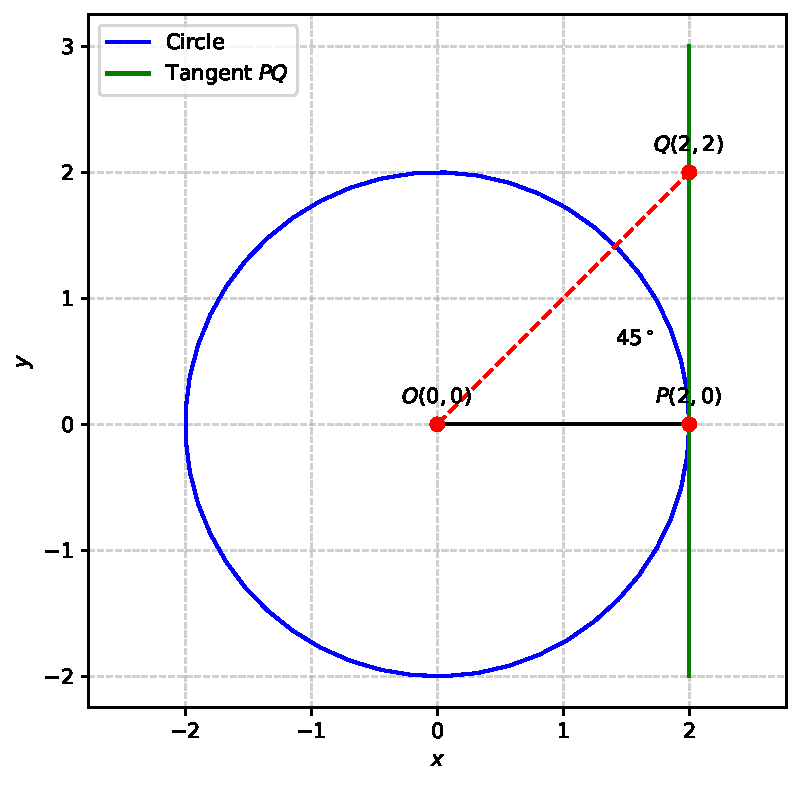
\includegraphics[width=0.70\linewidth]{figs/cbXq6.pdf}
    \caption{Tangent $PQ$ and the isosceles triangle $OPQ$ with $\angle OQP=45^{\circ}$}
    \label{fig:EE26BTECH11218-cb_q6}
\end{figure}
\item Two concentric circles have radii $10$ cm and $6$ cm. Find the length of the chord of the larger circle which touches the smaller circle.
\hfill (CBSE~X~2021)
\\
\solution
With the common centre at the origin, from \eqref{eq:EE26BTECH11218-cb-circle} the circles have
\begin{align}
\vec{V} = \vec{I}, \quad \vec{u} = \vec{0}, \quad f_1 = -100 \text{ (larger)}, \quad f_2 = -36 \text{ (smaller)}
\end{align}
Choose the axes so that the chord is the line $\vec{x} = \vec{h}+\kappa\vec{m}$ with
\begin{align}
\vec{h} = \myvec{6 \\ 0}, \quad \vec{m} = \myvec{0 \\ 1}, \quad \vec{m}^{\top}\vec{h}=0
\end{align}
For the smaller circle, $\vec{m}^{\top}\brak{\vec{V}\vec{h}+\vec{u}} = 0$ and $g\brak{\vec{h}} = \norm{\vec{h}}^2 - 36 = 0$, so \eqref{eq:EE26BTECH11218-cb-chord} gives $\Delta = 0$ and the line is tangent. For the larger circle, $g\brak{\vec{h}} = 36-100 = -64$, $\vec{m}^{\top}\vec{V}\vec{m} = 1$, so from \eqref{eq:EE26BTECH11218-cb-kappa}
\begin{align}
\kappa = \frac{0 \pm \sqrt{0 + 64}}{1} = \pm 8
\implies \vec{x}_{1,2} = \myvec{6 \\ \pm 8}
\end{align}
Hence the length of the chord, from \eqref{eq:EE26BTECH11218-cb-chord}, is
\begin{align}
\norm{\vec{x}_1-\vec{x}_2} = \abs{8-\brak{-8}}\norm{\vec{m}} = 16 \text{ cm}
\end{align}
The following code verifies this in \figref{fig:EE26BTECH11218-cb_q7}.
\begin{lstlisting}[frame=single, basicstyle=\rmfamily, escapeinside={(*@}{@*)}]
(*@\makebox[\dimexpr\linewidth-2\fboxsep-2\fboxrule\relax][c]{codes/cbXq7.py}@*)
\end{lstlisting}
\begin{figure}[H]
    \centering
    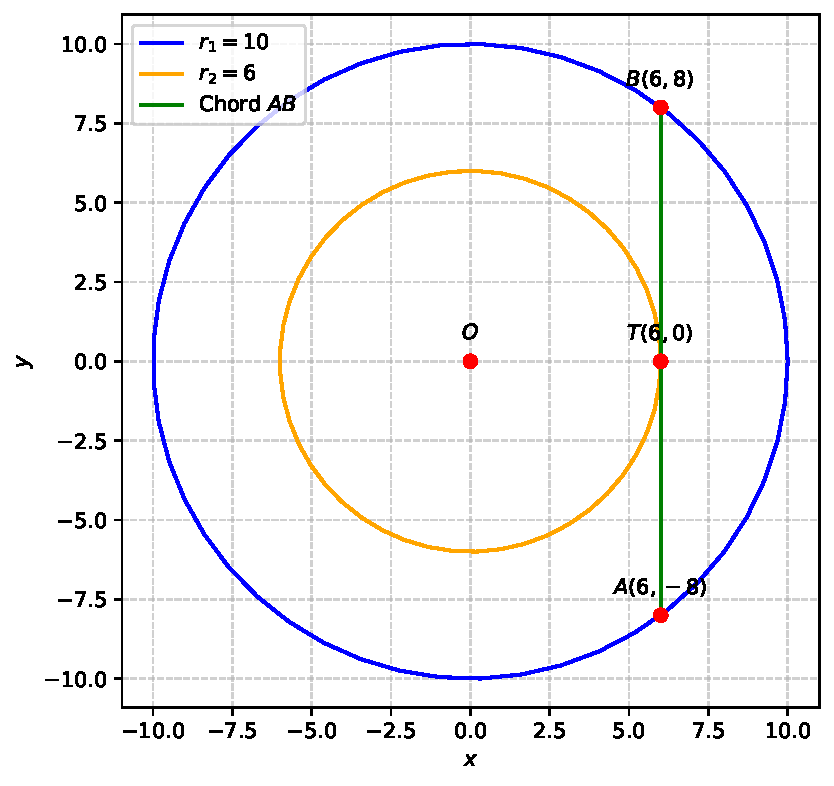
\includegraphics[width=0.70\linewidth]{figs/cbXq7.pdf}
    \caption{Chord of the larger circle touching the smaller circle}
    \label{fig:EE26BTECH11218-cb_q7}
\end{figure}
\item How many outcomes are possible when three dice are thrown together?
\hfill (CBSE~X~2021)
\\
\solution
For one die, the generating function of the outcomes is $x+x^2+\cdots+x^6$. For three dice, from \eqref{eq:EE26BTECH11218-cb-dice-count}, the number of outcomes with sum $n$ is the coefficient of $x^n$ in
\begin{align}
\brak{x+x^2+\cdots+x^6}^3 &= x^3 + 3x^4 + 6x^5 + 10x^6 + 15x^7 + 21x^8 \\
&\quad + 25x^9 + 27x^{10} + \cdots + x^{18}
\end{align}
and setting $x=1$ adds the counts of all sums,
\begin{align}
\brak{1+1+\cdots+1}^3 = 6^3 = 216
\end{align}
The following code verifies this in \figref{fig:EE26BTECH11218-cb_q16}.
\begin{lstlisting}[frame=single, basicstyle=\rmfamily, escapeinside={(*@}{@*)}]
(*@\makebox[\dimexpr\linewidth-2\fboxsep-2\fboxrule\relax][c]{codes/cbXq16.py}@*)
\end{lstlisting}
\begin{figure}[H]
    \centering
    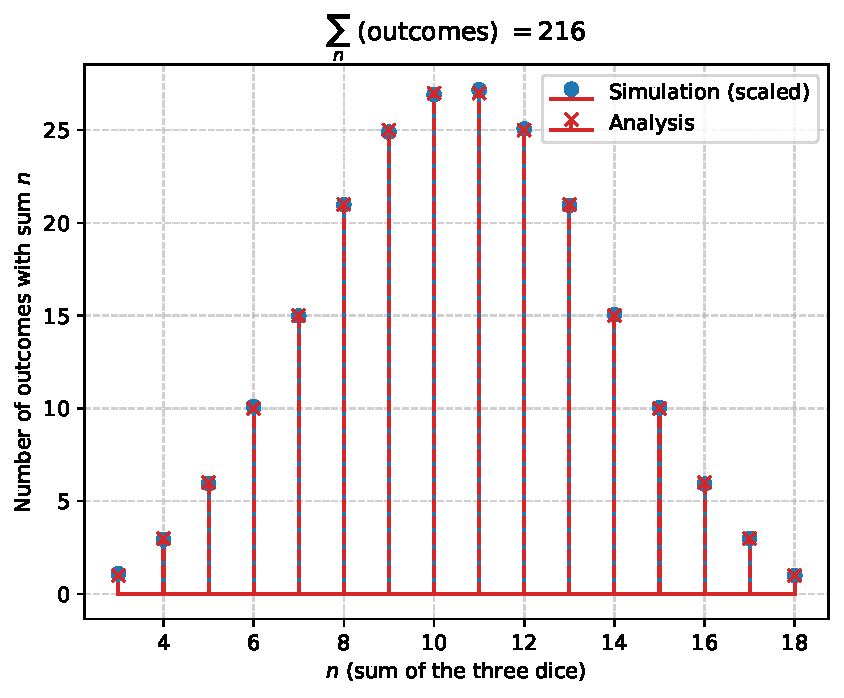
\includegraphics[width=0.70\linewidth]{figs/cbXq16.pdf}
    \caption{Number of outcomes for each sum of three dice: Simulation vs Analysis}
    \label{fig:EE26BTECH11218-cb_q16}
\end{figure}
\item The residents of a housing society decided to build two straight paths in the central park. Taking one corner of the park as origin and two mutually perpendicular lines as the axes, the paths are represented by $2x-3y=5$ and $-6x+9y=7$.
\hfill (CBSE~X~2021)

\begin{enumerate}[label=(\roman*), itemsep=0pt]
\item The two paths are
\begin{enumerate}[label=\alph*), itemsep=0pt]
    \begin{multicols}{2}
        \item intersecting
        \item overlapping
        \item parallel
        \item mutually perpendicular
    \end{multicols}
\end{enumerate}
\item Which of the following points lies on the line $2x-3y=5$?
\begin{enumerate}[label=\alph*), itemsep=0pt]
    \begin{multicols}{4}
        \item $\brak{-4,1}$
        \item $\brak{4,-1}$
        \item $\brak{4,1}$
        \item $\brak{-4,-1}$
    \end{multicols}
\end{enumerate}
\item If the line $-6x+9y=7$ intersects the $y$-axis at a point, its coordinates are
\begin{enumerate}[label=\alph*), itemsep=0pt]
    \begin{multicols}{4}
        \item $\brak{0,\frac{7}{9}}$
        \item $\brak{\frac{7}{9},0}$
        \item $\brak{-\frac{7}{6},0}$
        \item $\brak{0,-\frac{7}{6}}$
    \end{multicols}
\end{enumerate}
\item If a pair of equations $a_1x+b_1y+c_1=0$ and $a_2x+b_2y+c_2=0$ has a unique solution, then
\begin{enumerate}[label=\alph*), itemsep=0pt]
    \begin{multicols}{4}
        \item $\frac{a_1}{a_2}=\frac{b_1}{b_2}=\frac{c_1}{c_2}$
        \item $\frac{a_1}{a_2}\ne\frac{b_1}{b_2}$
        \item $\frac{a_1}{a_2}=\frac{b_1}{b_2}\ne\frac{c_1}{c_2}$
        \item $\frac{a_1}{a_2}\ne\frac{b_1}{b_2}\ne\frac{c_1}{c_2}$
    \end{multicols}
\end{enumerate}
\item If $\frac{a_1}{a_2}=\frac{b_1}{b_2}=\frac{c_1}{c_2}$, the two lines are
\begin{enumerate}[label=\alph*), itemsep=0pt]
    \begin{multicols}{4}
        \item parallel
        \item coincident
        \item intersecting
        \item perpendicular to each other
    \end{multicols}
\end{enumerate}
\end{enumerate}
\solution
The paths are the matrix equation \eqref{eq:EE26BTECH11218-cb-linsys} with
\begin{align}
\vec{A} = \myvec{2 & -3 \\ -6 & 9}, \quad \vec{b} = \myvec{5 \\ 7}
\end{align}
\textbf{(i)} The second row of $\vec{A}$ is $-3$ times the first, so $\mydet{\vec{A}} = 18-18 = 0$ and $\rank\brak{\vec{A}} = 1$. Applying $R_2 \to R_2+3R_1$ to the augmented matrix,
\begin{align}
\augvec{2}{1}{2 & -3 & 5 \\ -6 & 9 & 7} \xrightarrow{R_2 \to R_2+3R_1} \augvec{2}{1}{2 & -3 & 5 \\ 0 & 0 & 22}
\end{align}
so $\rank\brak{\vec{A}} = 1 < 2 = \rank\brak{\sbrak{\vec{A}\mid\vec{b}}}$. From \eqref{eq:EE26BTECH11218-cb-rank-cases} the system is inconsistent with parallel normals, so the paths are \textbf{parallel}: option (c). Their distance, writing the second line as $\vec{n}_1^{\top}\vec{x}=-\frac{7}{3}$ with $\vec{n}_1 = \myvec{2 \\ -3}$, is
\begin{align}
\frac{\abs{5-\brak{-\frac{7}{3}}}}{\norm{\vec{n}_1}} = \frac{22}{3\sqrt{13}} \approx 2.03
\end{align}
\textbf{(ii)} Evaluating $\vec{n}_1^{\top}\vec{x}_0$ for the four points gives $-11,\ 11,\ 5,\ -5$, and only $\brak{4,1}$ gives $5$: option (c).

\textbf{(iii)} On the $y$-axis $\vec{e}_1^{\top}\vec{x}=0$, so $9y=7$ and the point is $\brak{0,\frac{7}{9}}$: option (a).

\textbf{(iv)} A unique solution requires $\rank\brak{\vec{A}}=2$, i.e. $\mydet{\vec{A}} = a_1b_2-a_2b_1 \ne 0$. From \eqref{eq:EE26BTECH11218-cb-rank-cases} this is $\frac{a_1}{a_2}\ne\frac{b_1}{b_2}$: option (b).

\textbf{(v)} If the rows are proportional, $\rank\brak{\vec{A}} = \rank\brak{\sbrak{\vec{A}\mid\vec{b}}} = 1$, so the system has infinitely many solutions and the lines are \textbf{coincident}: option (b).

The following code verifies the results in \figref{fig:EE26BTECH11218-cb_q17}.
\begin{lstlisting}[frame=single, basicstyle=\rmfamily, escapeinside={(*@}{@*)}]
(*@\makebox[\dimexpr\linewidth-2\fboxsep-2\fboxrule\relax][c]{codes/cbXq17.py}@*)
\end{lstlisting}
\begin{figure}[H]
    \centering
    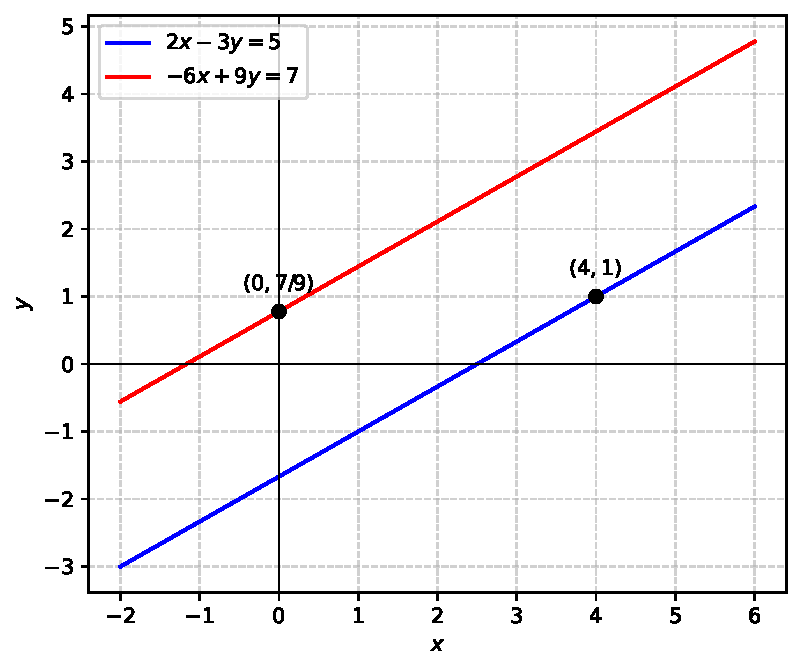
\includegraphics[width=0.70\linewidth]{figs/cbXq17.pdf}
    \caption{The parallel paths $2x-3y=5$ and $-6x+9y=7$}
    \label{fig:EE26BTECH11218-cb_q17}
\end{figure}
\item The time taken (in seconds) by a group of students to complete a race is recorded as follows.
\begin{center}
\begin{tabular}{|c|c|c|c|c|c|}
\hline
Time (s) & $0$--$20$ & $20$--$40$ & $40$--$60$ & $60$--$80$ & $80$--$100$ \\ \hline
Students & $1$ & $4$ & $3$ & $7$ & $5$ \\ \hline
\end{tabular}
\end{center}
\hfill (CBSE~X~2021)

\begin{enumerate}[label=(\roman*), itemsep=0pt]
\item The class mark of the modal class is
\begin{enumerate}[label=\alph*), itemsep=0pt]
    \begin{multicols}{4}
        \item $60$
        \item $70$
        \item $80$
        \item $140$
    \end{multicols}
\end{enumerate}
\item The mode of the given data is
\begin{enumerate}[label=\alph*), itemsep=0pt]
    \begin{multicols}{4}
        \item $70.33$
        \item $71.33$
        \item $72.33$
        \item $73.33$
    \end{multicols}
\end{enumerate}
\item The median class of the given data is
\begin{enumerate}[label=\alph*), itemsep=0pt]
    \begin{multicols}{4}
        \item $20$--$40$
        \item $40$--$60$
        \item $80$--$100$
        \item $60$--$80$
    \end{multicols}
\end{enumerate}
\item The sum of the lower limits of the median class and the modal class is
\begin{enumerate}[label=\alph*), itemsep=0pt]
    \begin{multicols}{4}
        \item $80$
        \item $140$
        \item $120$
        \item $100$
    \end{multicols}
\end{enumerate}
\item The median time (in seconds) of the given data is
\begin{enumerate}[label=\alph*), itemsep=0pt]
    \begin{multicols}{4}
        \item $65.7$
        \item $85.7$
        \item $45.7$
        \item $25.7$
    \end{multicols}
\end{enumerate}
\end{enumerate}
\solution
Here $h=20$, $N=\sum_i f_i = 20$, and the cumulative frequencies are
\begin{align}
F_i = 1,\ 5,\ 8,\ 15,\ 20
\end{align}
\textbf{(i)} The largest frequency is $7$, so the modal class is $60$--$80$ with class mark $\frac{60+80}{2}=70$: option (b).

\textbf{(ii)} With $l=60$, $f_0=3$, $f_1=7$, $f_2=5$, the two lines of the histogram construction pass through
\begin{align}
\vec{A}_1 = \myvec{60 \\ 3},\ \vec{B}_1 = \myvec{80 \\ 7}, \qquad \vec{A}_2 = \myvec{60 \\ 7},\ \vec{B}_2 = \myvec{80 \\ 5}
\end{align}
The direction vectors are $\vec{m}_1 = \myvec{20 \\ 4}$, $\vec{m}_2 = \myvec{20 \\ -2}$, with normals obtained by a $90^{\circ}$ rotation, $\vec{n}_i = \myvec{0 & 1 \\ -1 & 0}\vec{m}_i$, so that
\begin{align}
\myvec{4 & -20 \\ -2 & -20}\vec{x} = \myvec{\vec{n}_1^{\top}\vec{A}_1 \\ \vec{n}_2^{\top}\vec{A}_2} = \myvec{180 \\ -260}
\implies \vec{x} = \myvec{73.33 \\ 5.67}
\end{align}
Its abscissa is the mode, which agrees with \eqref{eq:EE26BTECH11218-cb-mode}
\begin{align}
60 + \frac{7-3}{14-3-5}\times 20 = 73.33
\end{align}
option (d).

\textbf{(iii)} Since $\frac{N}{2}=10$ and $F_3 = 8 < 10 \le 15 = F_4$, the median class is $60$--$80$: option (d).

\textbf{(iv)} The lower limits of both classes are $60$, so the sum is $120$: option (c).

\textbf{(v)} From \eqref{eq:EE26BTECH11218-cb-median}, with $l=60$, $F_{k-1}=8$, $f_k=7$,
\begin{align}
\text{Median} = 60 + \frac{10-8}{7}\times 20 = 60+\frac{40}{7} \approx 65.7
\end{align}
option (a). The following code verifies the mode as a line intersection and the median as the root of the ogive in \figref{fig:EE26BTECH11218-cb_q19}.
\begin{lstlisting}[frame=single, basicstyle=\rmfamily, escapeinside={(*@}{@*)}]
(*@\makebox[\dimexpr\linewidth-2\fboxsep-2\fboxrule\relax][c]{codes/cbXq19.py}@*)
\end{lstlisting}
\begin{figure}[H]
    \centering
    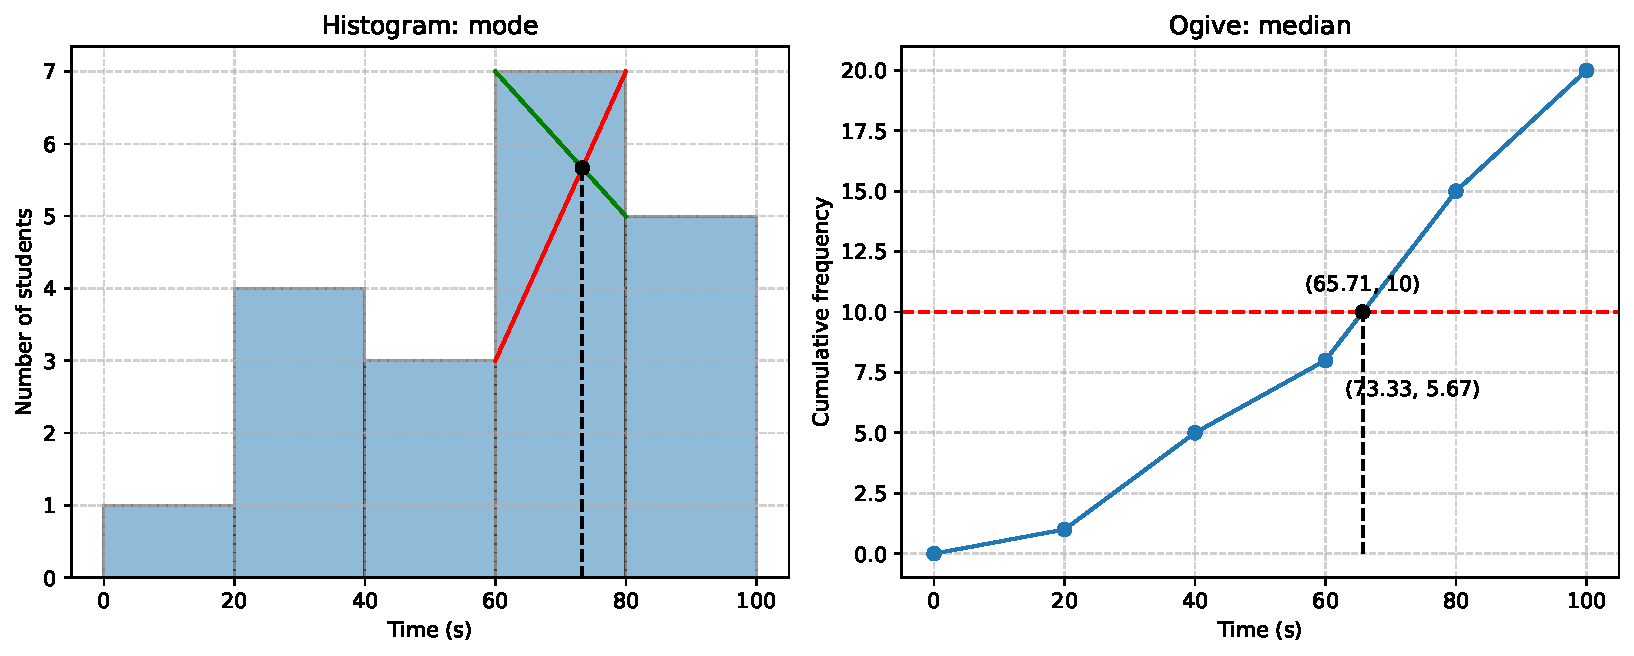
\includegraphics[width=0.95\linewidth]{figs/cbXq19.pdf}
    \caption{Histogram construction for the mode and ogive for the median}
    \label{fig:EE26BTECH11218-cb_q19}
\end{figure}
\item Twenty identical cards are numbered $1$ to $20$ and placed in a box. One card is drawn at random.
\hfill (CBSE~X~2021)

\begin{enumerate}[label=(\roman*), itemsep=0pt]
\item The probability that the number on the card is an odd prime number is
\begin{enumerate}[label=\alph*), itemsep=0pt]
    \begin{multicols}{4}
        \item $\frac{3}{5}$
        \item $\frac{2}{5}$
        \item $\frac{9}{20}$
        \item $\frac{7}{20}$
    \end{multicols}
\end{enumerate}
\item The probability that the number on the card is a composite number is
\begin{enumerate}[label=\alph*), itemsep=0pt]
    \begin{multicols}{4}
        \item $\frac{11}{20}$
        \item $\frac{3}{5}$
        \item $\frac{4}{5}$
        \item $\frac{1}{2}$
    \end{multicols}
\end{enumerate}
\item The probability that the number on the card is a multiple of $3$, $6$ and $9$ is
\begin{enumerate}[label=\alph*), itemsep=0pt]
    \begin{multicols}{4}
        \item $\frac{1}{20}$
        \item $\frac{1}{10}$
        \item $\frac{3}{20}$
        \item $0$
    \end{multicols}
\end{enumerate}
\item The probability that the number on the card is a multiple of $3$ and $7$ is
\begin{enumerate}[label=\alph*), itemsep=0pt]
    \begin{multicols}{4}
        \item $\frac{3}{10}$
        \item $\frac{1}{10}$
        \item $0$
        \item $\frac{2}{5}$
    \end{multicols}
\end{enumerate}
\item If all cards with odd numbers are removed and one card is drawn from the rest, the probability of a prime number is
\begin{enumerate}[label=\alph*), itemsep=0pt]
    \begin{multicols}{4}
        \item $\frac{1}{20}$
        \item $\frac{1}{10}$
        \item $0$
        \item $\frac{1}{5}$
    \end{multicols}
\end{enumerate}
\end{enumerate}
\solution
Let $\Omega = \cbrak{1,2,\dots,20}$ with $p_X\brak{n} = \frac{1}{20}$ and use \eqref{eq:EE26BTECH11218-cb-prob}. The primes in $\Omega$ are
\begin{align}
\cbrak{2,3,5,7,11,13,17,19}, \quad \abs{\cbrak{\text{primes}}} = 8
\end{align}
\textbf{(i)} Removing $2$ leaves $7$ odd primes, so $\pr{\text{odd prime}} = \frac{7}{20}$: option (d).

\textbf{(ii)} Neither $1$ nor a prime is composite, so $\abs{\cbrak{\text{composite}}} = 20-1-8 = 11$ and $\pr{\text{composite}}=\frac{11}{20}$: option (a).

\textbf{(iii)} A multiple of $3$, $6$ and $9$ is a multiple of $\operatorname{lcm}\brak{3,6,9}=18$. From \eqref{eq:EE26BTECH11218-cb-lcm}, the count is $\left\lfloor\frac{20}{18}\right\rfloor = 1$, so the probability is $\frac{1}{20}$: option (a).

\textbf{(iv)} $\operatorname{lcm}\brak{3,7}=21>20$, so the count is $\left\lfloor\frac{20}{21}\right\rfloor = 0$ and the probability is $0$: option (c).

\textbf{(v)} Let $E$ be the event ``even number'' and $S$ the event ``prime''. Then $\pr{E}=\frac{10}{20}$ and $SE=\cbrak{2}$, so
\begin{align}
\pr{S\mid E} = \frac{\pr{SE}}{\pr{E}} = \frac{1/20}{1/2} = \frac{1}{10}
\end{align}
option (b). The following code verifies these in \figref{fig:EE26BTECH11218-cb_q20}.
\begin{lstlisting}[frame=single, basicstyle=\rmfamily, escapeinside={(*@}{@*)}]
(*@\makebox[\dimexpr\linewidth-2\fboxsep-2\fboxrule\relax][c]{codes/cbXq20.py}@*)
\end{lstlisting}
\begin{figure}[H]
    \centering
    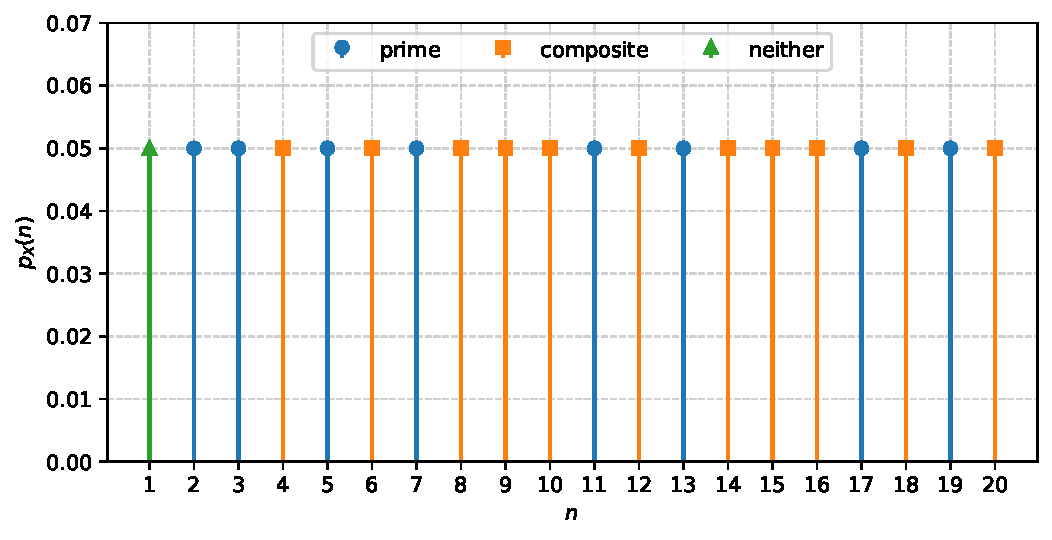
\includegraphics[width=0.70\linewidth]{figs/cbXq20.pdf}
    \caption{PMF of the card drawn, grouped as prime, composite and neither}
    \label{fig:EE26BTECH11218-cb_q20}
\end{figure}
\item Find the value of $k$ for which the system of equations $x+2y=5$ and $3x+ky+15=0$ has no solution.
\hfill (CBSE~X~2021)
\\
\solution
From \eqref{eq:EE26BTECH11218-cb-linsys},
\begin{align}
\myvec{1 & 2 \\ 3 & k}\myvec{x \\ y} = \myvec{5 \\ -15}
\end{align}
Applying Gaussian elimination to the augmented matrix,
\begin{align}
\augvec{2}{1}{1 & 2 & 5 \\ 3 & k & -15} \xrightarrow{R_2 \to R_2-3R_1} \augvec{2}{1}{1 & 2 & 5 \\ 0 & k-6 & -30}
\end{align}
If $k\ne6$, then $\rank\brak{\vec{A}}=2$ and the solution is unique. If $k=6$, then $\rank\brak{\vec{A}}=1$ while the last row of the augmented matrix is $\myvec{0 & 0 & -30}$, so $\rank\brak{\sbrak{\vec{A}\mid\vec{b}}}=2$. From \eqref{eq:EE26BTECH11218-cb-rank-cases},
\begin{align}
\rank\brak{\vec{A}} < \rank\brak{\sbrak{\vec{A}\mid\vec{b}}} \implies k = 6
\end{align}
This agrees with $\frac{1}{3}=\frac{2}{k}\ne\frac{-5}{15}$ at $k=6$. The following code verifies this in \figref{fig:EE26BTECH11218-cb_q22}.
\begin{lstlisting}[frame=single, basicstyle=\rmfamily, escapeinside={(*@}{@*)}]
(*@\makebox[\dimexpr\linewidth-2\fboxsep-2\fboxrule\relax][c]{codes/cbXq22.py}@*)
\end{lstlisting}
\begin{figure}[H]
    \centering
    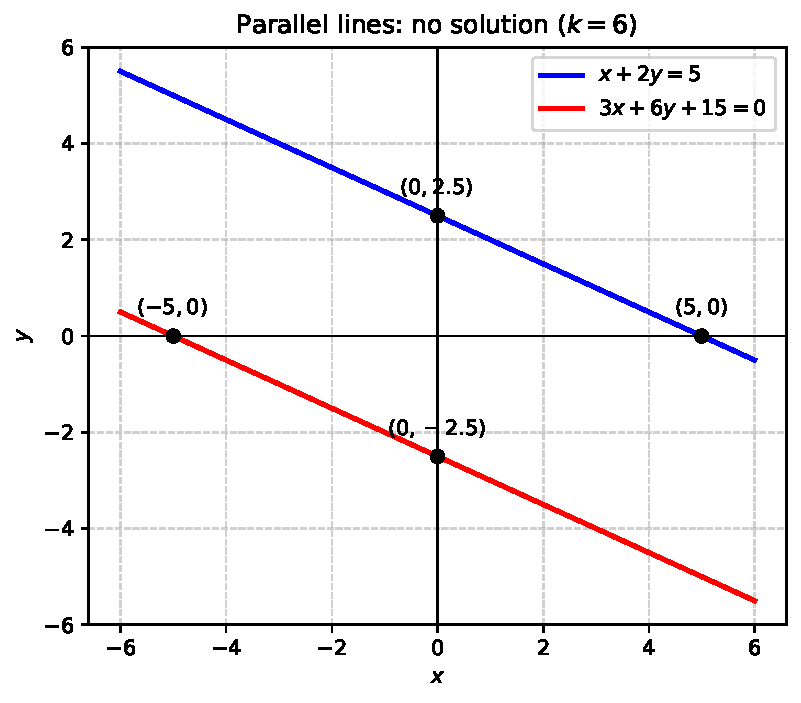
\includegraphics[width=0.70\linewidth]{figs/cbXq22.pdf}
    \caption{Parallel lines $x+2y=5$ and $3x+6y+15=0$ ($k=6$): no solution}
    \label{fig:EE26BTECH11218-cb_q22}
\end{figure}
\item $ABC$ is a right triangle, right-angled at $B$, with $BC=6$ cm and $AB=8$ cm. A circle with centre $O$ and radius $r$ cm is inscribed in $\triangle ABC$. Find the value of $r$.
\hfill (CBSE~X~2021)
\\
\solution
Taking $B$ as the origin with $BC$ and $BA$ along the axes,
\begin{align}
\vec{A} = \myvec{0 \\ 8}, \quad \vec{B} = \myvec{0 \\ 0}, \quad \vec{C} = \myvec{6 \\ 0}
\end{align}
The sides are $a=BC=6$, $c=AB=8$ and $b=CA=\norm{\vec{C}-\vec{A}}=10$. From \eqref{eq:EE26BTECH11218-cb-incircle},
\begin{align}
\vec{I} = \frac{6\myvec{0 \\ 8} + 10\myvec{0 \\ 0} + 8\myvec{6 \\ 0}}{24} = \myvec{2 \\ 2}, \qquad
r = \frac{\Delta}{s} = \frac{\frac{1}{2}\cdot6\cdot8}{12} = 2
\end{align}
Using the linear system \eqref{eq:EE26BTECH11218-cb-incircle-sys} with the inward unit normals of $AB$, $BC$ and $CA$ ($4x+3y=24$),
\begin{align}
\myvec{1 & 0 & -1 \\ 0 & 1 & -1 \\ -0.8 & -0.6 & -1}\myvec{x \\ y \\ r} = \myvec{0 \\ 0 \\ -4.8}
\implies \myvec{x \\ y \\ r} = \myvec{2 \\ 2 \\ 2}
\end{align}
Also, from \eqref{eq:EE26BTECH11218-cb-incircle-right}, $r = \frac{6+8-10}{2} = 2$.
\begin{align}
\therefore r = 2 \text{ cm}
\end{align}
The points of contact are $\vec{P}=\myvec{0 \\ 2}$, $\vec{Q}=\myvec{2 \\ 0}$ and $\vec{R}=\myvec{3.6 \\ 3.2}$. The following code verifies this in \figref{fig:EE26BTECH11218-cb_q25}.
\begin{lstlisting}[frame=single, basicstyle=\rmfamily, escapeinside={(*@}{@*)}]
(*@\makebox[\dimexpr\linewidth-2\fboxsep-2\fboxrule\relax][c]{codes/cbXq25.py}@*)
\end{lstlisting}
\begin{figure}[H]
    \centering
    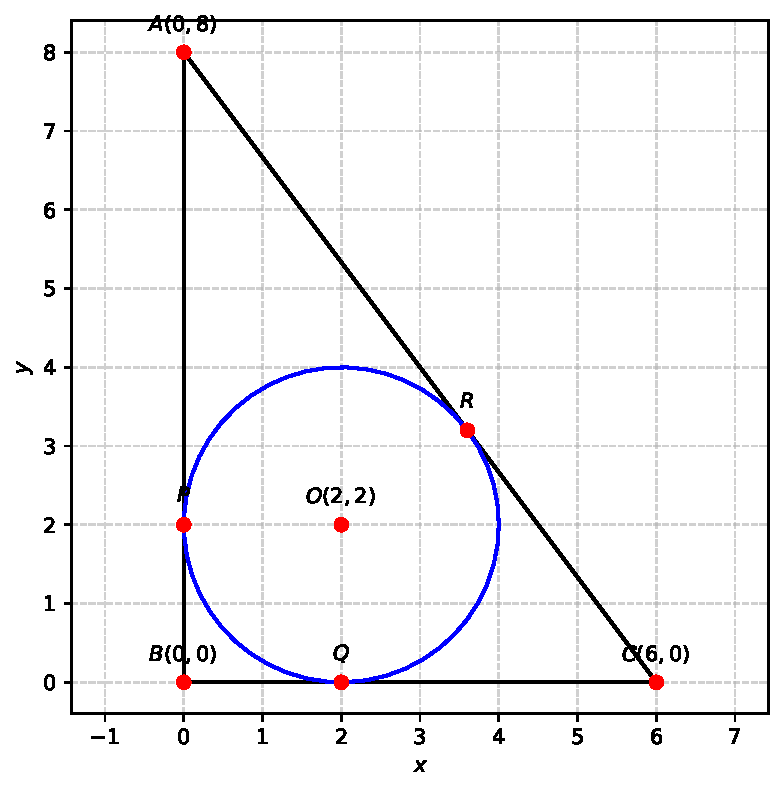
\includegraphics[width=0.70\linewidth]{figs/cbXq25.pdf}
    \caption{Incircle of the right triangle $ABC$ with $r=2$}
    \label{fig:EE26BTECH11218-cb_q25}
\end{figure}
\item Divide the polynomial $f\brak{x} = 5x^3+10x^2-30x-15$ by the polynomial $g\brak{x} = x^2+1+x$ and hence find the quotient and the remainder.
\hfill (CBSE~X~2021)
\\
\solution
From \eqref{eq:EE26BTECH11218-cb-division}, let $q\brak{x}=q_1x+q_0$ and $r\brak{x}=r_1x+r_0$. Then
\begin{align}
q\brak{x}g\brak{x} + r\brak{x} = q_1x^3 + \brak{q_1+q_0}x^2 + \brak{q_1+q_0+r_1}x + \brak{q_0+r_0}
\end{align}
Comparing coefficients with $f\brak{x}$ gives the matrix equation
\begin{align}
\myvec{1 & 0 & 0 & 0 \\ 1 & 1 & 0 & 0 \\ 1 & 1 & 1 & 0 \\ 0 & 1 & 0 & 1}\myvec{q_1 \\ q_0 \\ r_1 \\ r_0} = \myvec{5 \\ 10 \\ -30 \\ -15}
\implies \myvec{q_1 \\ q_0 \\ r_1 \\ r_0} = \myvec{5 \\ 5 \\ -40 \\ -20}
\end{align}
Verifying the remainder with \eqref{eq:EE26BTECH11218-cb-remainder}: the roots of $g$ are $\omega,\omega^2$ with $\omega^3=1$ and $\omega^2=-1-\omega$, so
\begin{align}
f\brak{\omega} = 5 + 10\omega^2 - 30\omega - 15 = -20-40\omega = r\brak{\omega}
\end{align}
and similarly for $\omega^2$, which gives $r\brak{x}=-40x-20$.
\begin{align}
\therefore q\brak{x} = 5x+5, \quad r\brak{x} = -40x-20
\end{align}
The following code verifies this in \figref{fig:EE26BTECH11218-cb_q27}.
\begin{lstlisting}[frame=single, basicstyle=\rmfamily, escapeinside={(*@}{@*)}]
(*@\makebox[\dimexpr\linewidth-2\fboxsep-2\fboxrule\relax][c]{codes/cbXq27.py}@*)
\end{lstlisting}
\begin{figure}[H]
    \centering
    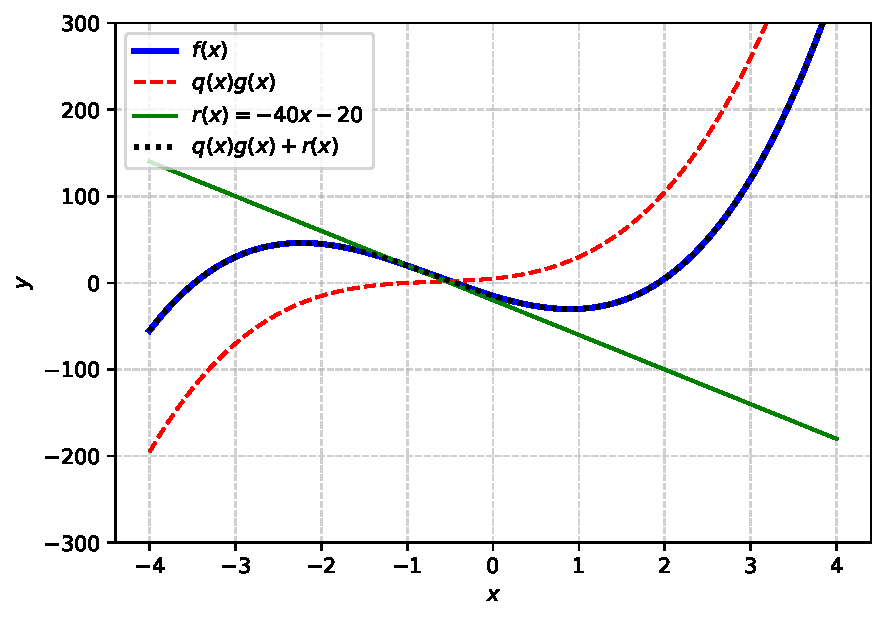
\includegraphics[width=0.70\linewidth]{figs/cbXq27.pdf}
    \caption{$f\brak{x}$ and $q\brak{x}g\brak{x}+r\brak{x}$ coincide}
    \label{fig:EE26BTECH11218-cb_q27}
\end{figure}
\item Water is being pumped out through a circular pipe whose internal diameter is $8$ cm. If the rate of flow of water is $80$ cm/s, how many litres of water are pumped out through this pipe in one hour?
\hfill (CBSE~X~2021)
\\
\solution
Here $R=4$ cm, $v=80$ cm/s and $T=3600$ s. From \eqref{eq:EE26BTECH11218-cb-flux},
\begin{align}
Q &= \int_0^{2\pi}\int_0^4 80\rho\,d\rho\,d\theta = 80\cdot2\pi\cdot8 = 1280\pi \text{ cm}^3/\text{s} \\
V &= \int_0^{3600} Q\,dt = 1280\pi\times3600 = 4608000\pi \text{ cm}^3
\end{align}
Since $1\text{ L}=1000\text{ cm}^3$,
\begin{align}
V = 4608\pi \text{ L} \approx 14476.46 \text{ L}
\end{align}
(with $\pi=\frac{22}{7}$, $V \approx 14482.29$ L). The following code verifies this in \figref{fig:EE26BTECH11218-cb_q34}.
\begin{lstlisting}[frame=single, basicstyle=\rmfamily, escapeinside={(*@}{@*)}]
(*@\makebox[\dimexpr\linewidth-2\fboxsep-2\fboxrule\relax][c]{codes/cbXq34.py}@*)
\end{lstlisting}
\begin{figure}[H]
    \centering
    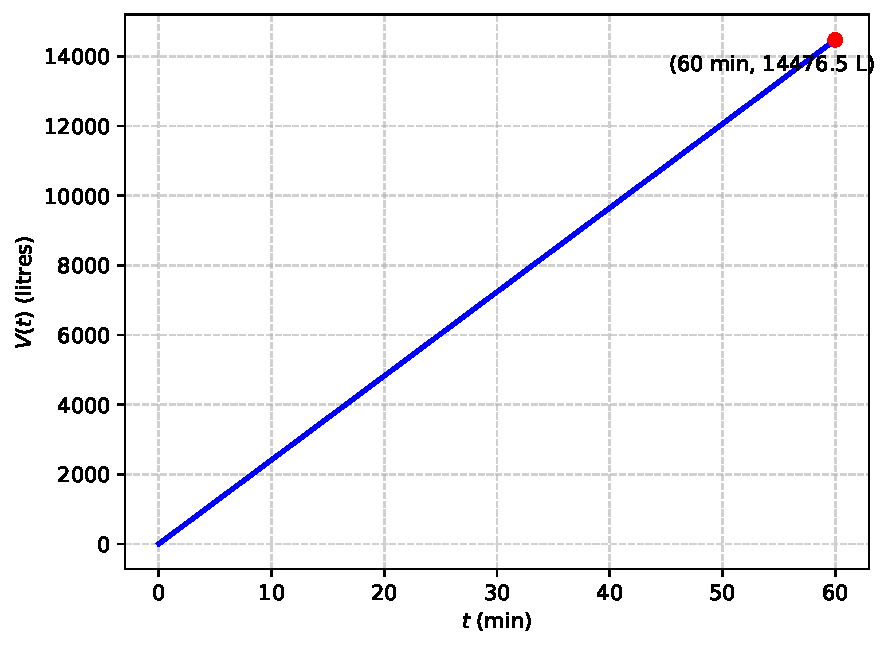
\includegraphics[width=0.70\linewidth]{figs/cbXq34.pdf}
    \caption{Volume pumped out versus time}
    \label{fig:EE26BTECH11218-cb_q34}
\end{figure}
\item A man on the top of a vertical tower observes a car moving at a uniform speed coming directly towards it. If it takes $18$ minutes for the angle of depression to change from $30^{\circ}$ to $60^{\circ}$, how soon after this will the car reach the tower?
\hfill (CBSE~X~2021)
\\
\solution
Let the tower have height $h$ and let $x\brak{t}$ be the horizontal distance of the car from its foot, with $t=0$ at the first observation. From \eqref{eq:EE26BTECH11218-cb-depression},
\begin{align}
x\brak{0} = h\cot30^{\circ} = \sqrt{3}h, \qquad x\brak{18} = h\cot60^{\circ} = \frac{h}{\sqrt{3}}
\end{align}
Using \eqref{eq:EE26BTECH11218-cb-uniform} and \eqref{eq:EE26BTECH11218-cb-uniform-sys} with $t_1=0$, $t_2=18$,
\begin{align}
\myvec{1 & 0 \\ 1 & -18}\myvec{x_0 \\ v} = \myvec{\sqrt{3}h \\ \frac{h}{\sqrt{3}}}
\implies x_0 = \sqrt{3}h, \quad v = \frac{1}{18}\brak{\sqrt{3}-\frac{1}{\sqrt{3}}}h = \frac{h}{9\sqrt{3}}
\end{align}
The car reaches the tower when $x\brak{t}=0$, that is after a further time
\begin{align}
t^{*} = \frac{x\brak{18}}{v} = \frac{h/\sqrt{3}}{h/\brak{9\sqrt{3}}} = 9 \text{ minutes}
\end{align}
which is independent of $h$. The following code verifies this in \figref{fig:EE26BTECH11218-cb_q35}.
\begin{lstlisting}[frame=single, basicstyle=\rmfamily, escapeinside={(*@}{@*)}]
(*@\makebox[\dimexpr\linewidth-2\fboxsep-2\fboxrule\relax][c]{codes/cbXq35.py}@*)
\end{lstlisting}
\begin{figure}[H]
    \centering
    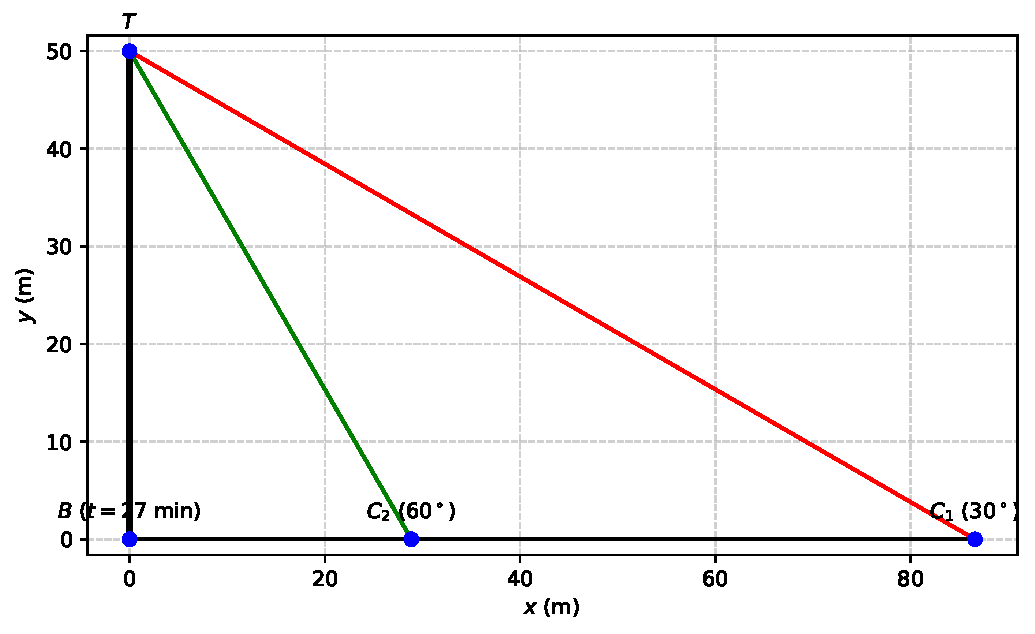
\includegraphics[width=0.70\linewidth]{figs/cbXq35.pdf}
    \caption{Car approaching the tower: angles of depression $30^{\circ}$ and $60^{\circ}$}
    \label{fig:EE26BTECH11218-cb_q35}
\end{figure}
\end{enumerate}

\newpage
\section{CBSE XII \cbxiiyear}
\subsection{Formulae}
\begin{enumerate}[label=\thesubsection.\arabic*, ref=\thesubsection.\theenumi,itemsep=1.5em]

\item (Independent Events and Sum of Random Variables) If $X$ and $Y$ are independent, that is, the events $\cbrak{X=x}$ and $\cbrak{Y=y}$ are independent for all $x,y$, with PMFs $p_X$ and $p_Y$,
\begin{align}
p_{X,Y}\brak{x,y} = p_X\brak{x}p_Y\brak{y}, \qquad p_{X+Y}\brak{n} = \sum_{k}p_X\brak{k}p_Y\brak{n-k}
\label{eq:EE26BTECH11218-cb12-conv}
\end{align}
and for independent events $E_i$ with $\pr{E_i}=p_i$,
\begin{align}
\pr{\text{at least one } E_i \text{ occurs}} = 1-\prod_i\brak{1-p_i}
\label{eq:EE26BTECH11218-cb12-atleast}
\end{align}
\solution Independence of the events $\cbrak{X=x}$ and $\cbrak{Y=y}$ factorises the joint PMF. The event $\cbrak{X+Y=n}$ is the disjoint union of $\cbrak{X=k,\,Y=n-k}$ over $k$, which gives the convolution. At least one event occurs iff the sum of the indicators is nonzero, and $\pr{\text{none}}=\prod_i\brak{1-p_i}$.

\item (Binomial Distribution) The number $X$ of successes in $n$ independent trials with success probability $p$ has
\begin{align}
p_X\brak{k} &= \binom{n}{k}p^k\brak{1-p}^{n-k}, \quad k=0,1,\dots,n \nonumber \\
E\sbrak{X} &= np, \quad \mathrm{var}\brak{X}=np\brak{1-p}
\label{eq:EE26BTECH11218-cb12-binom}
\end{align}
\solution One trial has the PMF $\brak{1-p,\ p}$, whose generating function is $1-p+px$. By \eqref{eq:EE26BTECH11218-cb12-conv} the PMF of the sum of $n$ trials is the $n$-fold convolution, that is, the coefficients of $\brak{1-p+px}^n$, which are $\binom{n}{k}p^k\brak{1-p}^{n-k}$ by the binomial theorem. The mean and variance add over the independent trials.

\item (Hypergeometric Distribution) Draw $n$ items without replacement from $M$ items, of which $K$ are of one kind. The number $X$ of items of that kind has
\begin{align}
p_X\brak{k} = \frac{\binom{K}{k}\binom{M-K}{n-k}}{\binom{M}{n}}, \qquad E\sbrak{X} = \frac{nK}{M}
\label{eq:EE26BTECH11218-cb12-hyper}
\end{align}
\solution All $\binom{M}{n}$ subsets of size $n$ are equally likely, and those with exactly $k$ items of the first kind can be chosen in $\binom{K}{k}\binom{M-K}{n-k}$ ways. Writing $X=\sum_{i=1}^{n}X_i$, where $X_i$ indicates that the $i$-th draw is of the first kind, symmetry gives $\pr{X_i=1}=\frac{K}{M}$ and hence the mean.

\item (Total Probability and Bayes' Theorem) If $B_1,\dots,B_m$ partition the sample space and $E$ is an event,
\begin{align}
\pr{B_j\mid E} = \frac{\pr{E\mid B_j}\pr{B_j}}{\sum_{i}\pr{E\mid B_i}\pr{B_i}}
\label{eq:EE26BTECH11218-cb12-bayes}
\end{align}
\solution $\pr{B_jE} = \pr{E\mid B_j}\pr{B_j} = \pr{B_j\mid E}\pr{E}$, and $\pr{E}=\sum_i\pr{EB_i} = \sum_i\pr{E\mid B_i}\pr{B_i}$.

\item (Lines in Space) A line through $\vec{a}$ with direction $\vec{m}$ is $\vec{x}=\vec{a}+\kappa\vec{m}$. The symmetric form
\begin{align}
\frac{x-x_0}{d_1} = \frac{y-y_0}{d_2} = \frac{z-z_0}{d_3} \implies \vec{m} = \myvec{d_1 \\ d_2 \\ d_3}
\label{eq:EE26BTECH11218-cb12-symm}
\end{align}
A condition such as $x=5$ means that coordinate is constant, so that component of $\vec{m}$ is $0$. The angle $\theta$ between two lines is the angle between their directions, and they are perpendicular iff
\begin{align}
\cos\theta = \frac{\vec{m}_1^{\top}\vec{m}_2}{\norm{\vec{m}_1}\norm{\vec{m}_2}} = 0 \iff \vec{m}_1^{\top}\vec{m}_2 = 0
\label{eq:EE26BTECH11218-cb12-perp}
\end{align}
\solution In the symmetric form, the point $\brak{x_0+\kappa d_1,\ y_0+\kappa d_2,\ z_0+\kappa d_3}$ moves along $\vec{m}$ as $\kappa$ varies, so $\vec{m}$ is the direction. A constant coordinate does not change with $\kappa$, so the corresponding component is $0$.

\item (Cross Product, Area and Collinearity) $\norm{\vec{u}\times\vec{v}}$ is the area of the parallelogram on $\vec{u},\vec{v}$, and $\vec{u}\times\vec{v}=\vec{0}$ iff $\vec{u}\parallel\vec{v}$. For three points,
\begin{align}
\brak{\vec{b}-\vec{a}}\times\brak{\vec{c}-\vec{a}} = \vec{b}\times\vec{c}+\vec{c}\times\vec{a}+\vec{a}\times\vec{b}
\label{eq:EE26BTECH11218-cb12-cross}
\end{align}
The area of the triangle is half the norm of this vector, and the points are collinear iff it is $\vec{0}$.
\solution By bilinearity,
\begin{align}
\brak{\vec{b}-\vec{a}}\times\brak{\vec{c}-\vec{a}} = \vec{b}\times\vec{c} - \vec{b}\times\vec{a} - \vec{a}\times\vec{c} + \vec{a}\times\vec{a}
\end{align}
and $\vec{a}\times\vec{a}=\vec{0}$, $-\vec{b}\times\vec{a}=\vec{a}\times\vec{b}$, $-\vec{a}\times\vec{c}=\vec{c}\times\vec{a}$.

\item (Determinants: Line and Area) The line through $\brak{x_1,y_1}$ and $\brak{x_2,y_2}$, and the area of a triangle with vertices $\brak{x_i,y_i}$, are, respectively,
\begin{align}
\mydet{x & y & 1 \\ x_1 & y_1 & 1 \\ x_2 & y_2 & 1} = 0, \qquad
\Delta = \frac{1}{2}\abs{\mydet{x_1 & y_1 & 1 \\ x_2 & y_2 & 1 \\ x_3 & y_3 & 1}}
\label{eq:EE26BTECH11218-cb12-det}
\end{align}
\solution The first determinant is affine in $\brak{x,y}$ and vanishes at both given points (two equal rows), so it is the equation of the line through them. For the second, subtracting row 3 from rows 1 and 2 and expanding along the last column,
\begin{align}
\mydet{x_1 & y_1 & 1 \\ x_2 & y_2 & 1 \\ x_3 & y_3 & 1} = \mydet{x_1-x_3 & y_1-y_3 \\ x_2-x_3 & y_2-y_3}
\end{align}
which is the signed area of the parallelogram on $\vec{x}_1-\vec{x}_3$ and $\vec{x}_2-\vec{x}_3$, twice the area of the triangle.

\item (Shortest Distance between Two Lines) For $\vec{x}=\vec{a}_1+s\vec{m}_1$ and $\vec{x}=\vec{a}_2+t\vec{m}_2$, let $\vec{M}=\myvec{\vec{m}_1 & \vec{m}_2}$ and $\vec{b}=\vec{a}_2-\vec{a}_1$. Then
\begin{align}
d = \min_{\vec{z}}\norm{\vec{M}\vec{z}-\vec{b}}, \quad \vec{M}^{\top}\vec{M}\vec{z} = \vec{M}^{\top}\vec{b}, \quad \vec{z}=\myvec{s \\ -t}
\label{eq:EE26BTECH11218-cb12-skew}
\end{align}
which is equivalent to
\begin{align}
d = \frac{\abs{\vec{b}^{\top}\brak{\vec{m}_1\times\vec{m}_2}}}{\norm{\vec{m}_1\times\vec{m}_2}}
\label{eq:EE26BTECH11218-cb12-skew-cross}
\end{align}
The lines intersect iff $d=0$.
\solution The distance between $\vec{a}_1+s\vec{m}_1$ and $\vec{a}_2+t\vec{m}_2$ is $\norm{s\vec{m}_1-t\vec{m}_2-\vec{b}}=\norm{\vec{M}\vec{z}-\vec{b}}$. It is minimum when the residual is orthogonal to both columns of $\vec{M}$ (the normal equations). The residual is then perpendicular to $\vec{m}_1$ and $\vec{m}_2$, so it is along $\vec{m}_1\times\vec{m}_2$ and equals the projection of $\vec{b}$ on that direction, which is \eqref{eq:EE26BTECH11218-cb12-skew-cross}.

\item (Planes through a Line of Intersection) The planes $\vec{n}_1^{\top}\vec{x}+e_1=0$ and $\vec{n}_2^{\top}\vec{x}+e_2=0$ meet in a line, and every plane through that line is
\begin{align}
\brak{\vec{n}_1+\lambda\vec{n}_2}^{\top}\vec{x} + \brak{e_1+\lambda e_2} = 0
\label{eq:EE26BTECH11218-cb12-pencil}
\end{align}
The distance of $\vec{n}^{\top}\vec{x}+e=0$ from the origin is
\begin{align}
\frac{\abs{e}}{\norm{\vec{n}}}
\label{eq:EE26BTECH11218-cb12-plane-dist}
\end{align}
\solution A point on both planes satisfies \eqref{eq:EE26BTECH11218-cb12-pencil} for every $\lambda$. The point of the plane nearest to the origin lies along the normal, $\vec{x}^{*}=-\frac{e}{\norm{\vec{n}}^2}\vec{n}$ (it satisfies $\vec{n}^{\top}\vec{x}^{*}+e=0$), and $\norm{\vec{x}^{*}}=\frac{\abs{e}}{\norm{\vec{n}}}$.

\item (Symmetric and Skew-Symmetric Parts) Every square matrix is $\vec{A}=\vec{S}+\vec{K}$ with
\begin{align}
\vec{S}=\frac{\vec{A}+\vec{A}^{\top}}{2}, \qquad \vec{K}=\frac{\vec{A}-\vec{A}^{\top}}{2}
\label{eq:EE26BTECH11218-cb12-symskew}
\end{align}
and $\vec{A}$ is symmetric iff $\vec{K}=\vec{0}$.
\solution $\vec{S}^{\top}=\vec{S}$, $\vec{K}^{\top}=-\vec{K}$ and $\vec{S}+\vec{K}=\vec{A}$. If $\vec{A}=\vec{A}^{\top}$, then $\vec{K}=\vec{0}$, and conversely.

\item (Idempotent Matrices and Matrix Polynomials) Let $\vec{A}^2=\vec{A}$ and let $p$ be a polynomial. Dividing $p\brak{\lambda}=q\brak{\lambda}\brak{\lambda^2-\lambda}+r_1\lambda+r_0$,
\begin{align}
p\brak{\vec{A}} = r_1\vec{A}+r_0\vec{I}, \qquad r_0=p\brak{0}, \quad r_1=p\brak{1}-p\brak{0}
\label{eq:EE26BTECH11218-cb12-idem}
\end{align}
\solution Since $\vec{A}^2-\vec{A}=\vec{0}$, the term $q\brak{\vec{A}}\brak{\vec{A}^2-\vec{A}}$ vanishes. Putting $\lambda=0$ and $\lambda=1$ (the roots of $\lambda^2-\lambda$) gives $p\brak{0}=r_0$ and $p\brak{1}=r_1+r_0$. Also, if $\vec{A}\vec{v}=\mu\vec{v}$ then $\mu^2=\mu$, so the eigenvalues of $\vec{A}$ are $0$ or $1$.

\item (Relations as Boolean Matrices) On a finite set $\cbrak{x_1,\dots,x_n}$ let $M_{ij}=1$ iff $x_iRx_j$. Then
\begin{align}
\text{reflexive} &\iff M_{ii}=1\ \forall i \nonumber \\
\text{symmetric} &\iff \vec{M}=\vec{M}^{\top} \nonumber \\
\text{transitive} &\iff \brak{\vec{M}^2>0}\subseteq\brak{\vec{M}>0}
\label{eq:EE26BTECH11218-cb12-relation}
\end{align}
If $L_{ik}=1$ when word $i$ contains letter $k$, then ``have a letter in common'' is $\vec{M}=\brak{\vec{L}\vec{L}^{\top}>0}$.
\solution $\brak{\vec{M}^2}_{ik}=\sum_jM_{ij}M_{jk}$ counts the $j$ with $x_iRx_jRx_k$, so it is positive iff a two-step chain exists, and transitivity requires $x_iRx_k$ for every such chain. Also, $\brak{\vec{L}\vec{L}^{\top}}_{ij}=\sum_kL_{ik}L_{jk}$ is the number of common letters, and it is symmetric by construction.

\item (Adjugate and Cayley-Hamilton) For a $2\times2$ matrix $\vec{A}$, the Cayley-Hamilton theorem states
\begin{align}
\vec{A}^2-\mathrm{tr}\brak{\vec{A}}\vec{A}+\mydet{\vec{A}}\vec{I}=\vec{0}
\label{eq:EE26BTECH11218-cb12-ch}
\end{align}
and the adjugate satisfies
\begin{align}
\mathrm{adj}\brak{\vec{A}} = \mathrm{tr}\brak{\vec{A}}\vec{I}-\vec{A}, \qquad \vec{A}\,\mathrm{adj}\brak{\vec{A}} = \mathrm{adj}\brak{\vec{A}}\,\vec{A} = \mydet{\vec{A}}\vec{I}
\label{eq:EE26BTECH11218-cb12-adj}
\end{align}
\solution For $\vec{A}=\myvec{a & b \\ c & d}$ the transposed cofactor matrix is $\myvec{d & -b \\ -c & a} = \brak{a+d}\vec{I}-\vec{A}$. By \eqref{eq:EE26BTECH11218-cb12-ch}, $\vec{A}\brak{\mathrm{tr}\brak{\vec{A}}\vec{I}-\vec{A}} = \mathrm{tr}\brak{\vec{A}}\vec{A}-\vec{A}^2 = \mydet{\vec{A}}\vec{I}$, and the other product is the same because $\vec{A}$ commutes with $\vec{I}$ and with itself. No inverse is used, so this holds even when $\mydet{\vec{A}}=0$.

\item (Improper Integral and Substitution) If $f$ is continuous on $\sbrak{a,b}$ except for an unbounded point at $b$,
\begin{align}
\int_a^bf\brak{x}dx = \lim_{c\to b^{-}}\int_a^cf\brak{x}dx
\label{eq:EE26BTECH11218-cb12-improper}
\end{align}
whenever the limit exists. With $x=\sin\theta$, a right triangle with hypotenuse $1$ gives $\tan\brak{\sin^{-1}x}=\frac{x}{\sqrt{1-x^2}}$ and $dx=\cos\theta\,d\theta$.

\item (Integration by Parts) $\int u\,dv = uv-\int v\,du$, and
\begin{align}
\int e^x\brak{f\brak{x}+f'\brak{x}}dx = e^xf\brak{x}+c
\label{eq:EE26BTECH11218-cb12-expf}
\end{align}
\solution With $u=f$ and $dv=e^xdx$, $\int e^xf\,dx = e^xf-\int e^xf'\,dx$. Adding $\int e^xf'\,dx$ to both sides gives \eqref{eq:EE26BTECH11218-cb12-expf}.

\item (First-Order Linear ODE) The equation $\diff{y}{x}+P\brak{x}y=Q\brak{x}$ has the integrating factor
\begin{align}
\mu\brak{x} = e^{\int P\,dx}, \qquad \diff{}{x}\brak{\mu y} = \mu Q
\label{eq:EE26BTECH11218-cb12-linode}
\end{align}
\solution By the product rule $\diff{}{x}\brak{\mu y} = \mu\diff{y}{x}+\mu'y$, which equals $\mu\brak{\diff{y}{x}+Py}$ iff $\mu'=P\mu$, that is $\mu=e^{\int P\,dx}$.

\item (Area between Curves) The area between $y=f_1\brak{x}$ (above) and $y=f_2\brak{x}$ on $\sbrak{a,b}$ is $\int_a^b\brak{f_1-f_2}dx$. For the region between $x=y^2$ and $x=4$, which is symmetric about the $x$-axis ($y=\pm\sqrt{x}$), the part with $x\le a$ has area
\begin{align}
A\brak{a} = \int_0^a2\sqrt{x}\,dx = \frac{4}{3}a^{3/2}
\label{eq:EE26BTECH11218-cb12-area}
\end{align}
and the line $x=a$ divides the region into two equal parts iff $A\brak{a}=\frac{1}{2}A\brak{4}$.

\item (Partial Fractions) A proper rational function with a repeated factor is
\begin{align}
\frac{p\brak{x}}{\brak{x-r}^2\brak{x-s}} = \frac{A}{x-r}+\frac{B}{\brak{x-r}^2}+\frac{C}{x-s}
\label{eq:EE26BTECH11218-cb12-partial}
\end{align}
where $A,B,C$ solve the linear system obtained by matching the coefficients of $p\brak{x}=A\brak{x-r}\brak{x-s}+B\brak{x-s}+C\brak{x-r}^2$. Then $\int\frac{dx}{x-r}=\ln\abs{x-r}$ and $\int\frac{dx}{\brak{x-r}^2}=-\frac{1}{x-r}$.
\end{enumerate}

\newpage
\subsection{Problems}
\providecommand{\cbxiiyear}{2021}
\begin{enumerate}[label=\thesubsection.\arabic*, ref=\thesubsection.\theenumi,itemsep=1.5em]

\item The probabilities of solving a specific question independently by $A$ and $B$ are $\frac{1}{3}$ and $\frac{1}{5}$ respectively. If both try to solve the question independently, the probability that the question is solved is
\begin{enumerate}[label=\alph*), itemsep=0pt]
    \begin{multicols}{4}
        \item $\frac{7}{15}$
        \item $\frac{8}{15}$
        \item $\frac{2}{15}$
        \item $\frac{14}{15}$
    \end{multicols}
\end{enumerate}
\hfill (CBSE~XII~\cbxiiyear)
\\
\solution
Let $X_A,X_B\in\cbrak{0,1}$ indicate that $A$ and $B$ solve the question, with PMFs
\begin{align}
\brak{p_A\brak{0},\ p_A\brak{1}} = \brak{\frac{2}{3},\ \frac{1}{3}}, \qquad \brak{p_B\brak{0},\ p_B\brak{1}} = \brak{\frac{4}{5},\ \frac{1}{5}}
\end{align}
From \eqref{eq:EE26BTECH11218-cb12-conv}, the PMF of $S=X_A+X_B$ is the convolution
\begin{align}
\brak{p_S\brak{0},\ p_S\brak{1},\ p_S\brak{2}} = \brak{\frac{8}{15},\ \frac{6}{15},\ \frac{1}{15}}
\end{align}
where $p_S\brak{1} = \frac{2}{3}\cdot\frac{1}{5}+\frac{1}{3}\cdot\frac{4}{5} = \frac{6}{15}$. The question is solved iff $S\ge1$, so
\begin{align}
\pr{S\ge1} = 1-p_S\brak{0} = 1-\frac{8}{15} = \frac{7}{15}
\end{align}
which agrees with \eqref{eq:EE26BTECH11218-cb12-atleast}, $1-\brak{1-\frac{1}{3}}\brak{1-\frac{1}{5}}$. Hence the answer is option (a). The following code verifies this in \figref{fig:EE26BTECH11218-cb12_q1}.
\begin{lstlisting}[frame=single, basicstyle=\rmfamily, escapeinside={(*@}{@*)}]
(*@\makebox[\dimexpr\linewidth-2\fboxsep-2\fboxrule\relax][c]{codes/cbXIIq1.py}@*)
\end{lstlisting}
\begin{figure}[H]
    \centering
    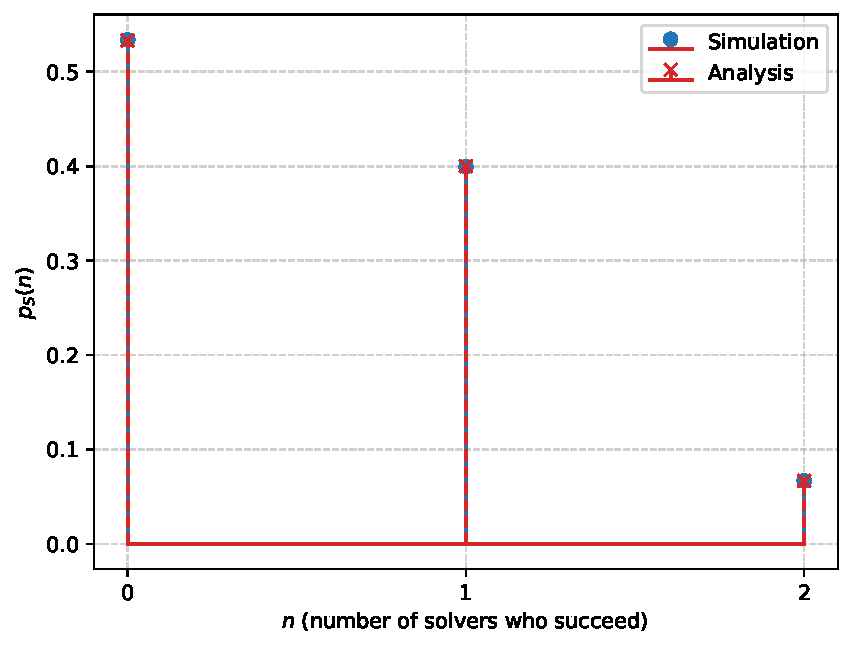
\includegraphics[width=0.70\linewidth]{figs/cbXIIq1.pdf}
    \caption{PMF of the number of solvers who succeed: Simulation vs Analysis}
    \label{fig:EE26BTECH11218-cb12_q1}
\end{figure}
\item If the two lines $L_1: x=5,\ \frac{y}{3-\alpha}=\frac{z}{-2}$ and $L_2: x=2,\ \frac{y}{-1}=\frac{z}{2-\alpha}$ are perpendicular, then the value of $\alpha$ is
\begin{enumerate}[label=\alph*), itemsep=0pt]
    \begin{multicols}{4}
        \item $\frac{2}{3}$
        \item $3$
        \item $4$
        \item $\frac{7}{3}$
    \end{multicols}
\end{enumerate}
\hfill (CBSE~XII~\cbxiiyear)
\\
\solution
From \eqref{eq:EE26BTECH11218-cb12-symm}, the directions of the lines are (the condition $x=5$ or $x=2$ means the $x$ component is $0$)
\begin{align}
\vec{m}_1 = \myvec{0 \\ 3-\alpha \\ -2}, \qquad \vec{m}_2 = \myvec{0 \\ -1 \\ 2-\alpha}
\end{align}
From \eqref{eq:EE26BTECH11218-cb12-perp}, the lines are perpendicular iff
\begin{align}
\vec{m}_1^{\top}\vec{m}_2 = -\brak{3-\alpha}-2\brak{2-\alpha} = 3\alpha-7 = 0 \implies \alpha = \frac{7}{3}
\end{align}
For $\alpha=\frac{2}{3},3,4$ the inner product is $-5,2,5$, all nonzero. Hence the answer is option (d). The following code verifies this in \figref{fig:EE26BTECH11218-cb12_q3}.
\begin{lstlisting}[frame=single, basicstyle=\rmfamily, escapeinside={(*@}{@*)}]
(*@\makebox[\dimexpr\linewidth-2\fboxsep-2\fboxrule\relax][c]{codes/cbXIIq3.py}@*)
\end{lstlisting}
\begin{figure}[H]
    \centering
    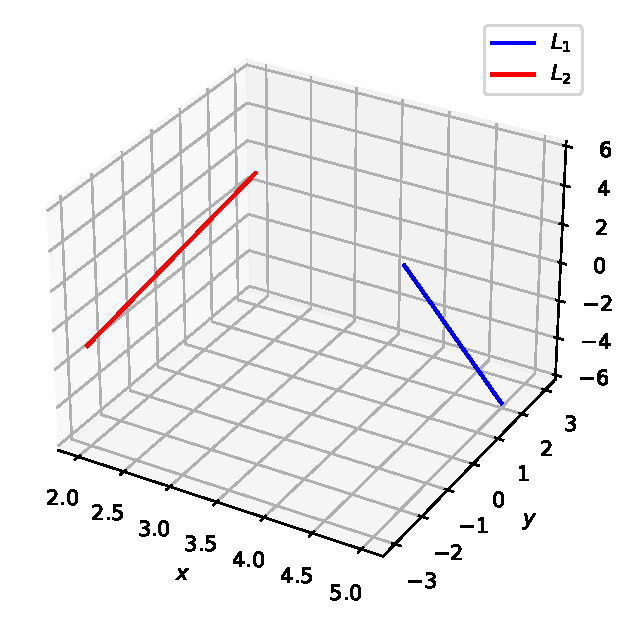
\includegraphics[width=0.70\linewidth]{figs/cbXIIq3.pdf}
    \caption{The perpendicular lines $L_1$ and $L_2$ for $\alpha=\frac{7}{3}$}
    \label{fig:EE26BTECH11218-cb12_q3}
\end{figure}
\item $\displaystyle\int_0^1\tan\brak{\sin^{-1}x}\,dx$ equals
\begin{enumerate}[label=\alph*), itemsep=0pt]
    \begin{multicols}{4}
        \item $2$
        \item $0$
        \item $-1$
        \item $1$
    \end{multicols}
\end{enumerate}
\hfill (CBSE~XII~\cbxiiyear)
\\
\solution
From \eqref{eq:EE26BTECH11218-cb12-improper}, $\tan\brak{\sin^{-1}x}=\frac{x}{\sqrt{1-x^2}}$, which is unbounded as $x\to1^{-}$, so the integral is improper. For $b<1$,
\begin{align}
\int_0^b\frac{x}{\sqrt{1-x^2}}dx = \sbrak{-\sqrt{1-x^2}}_0^b = 1-\sqrt{1-b^2}
\end{align}
and the limit is
\begin{align}
\lim_{b\to1^{-}}\brak{1-\sqrt{1-b^2}} = 1
\end{align}
The substitution $x=\sin\theta$ gives the same value, $\int_0^{\pi/2}\tan\theta\cos\theta\,d\theta=\int_0^{\pi/2}\sin\theta\,d\theta=1$. Hence the answer is option (d). The following code verifies this in \figref{fig:EE26BTECH11218-cb12_q6}.
\begin{lstlisting}[frame=single, basicstyle=\rmfamily, escapeinside={(*@}{@*)}]
(*@\makebox[\dimexpr\linewidth-2\fboxsep-2\fboxrule\relax][c]{codes/cbXIIq6.py}@*)
\end{lstlisting}
\begin{figure}[H]
    \centering
    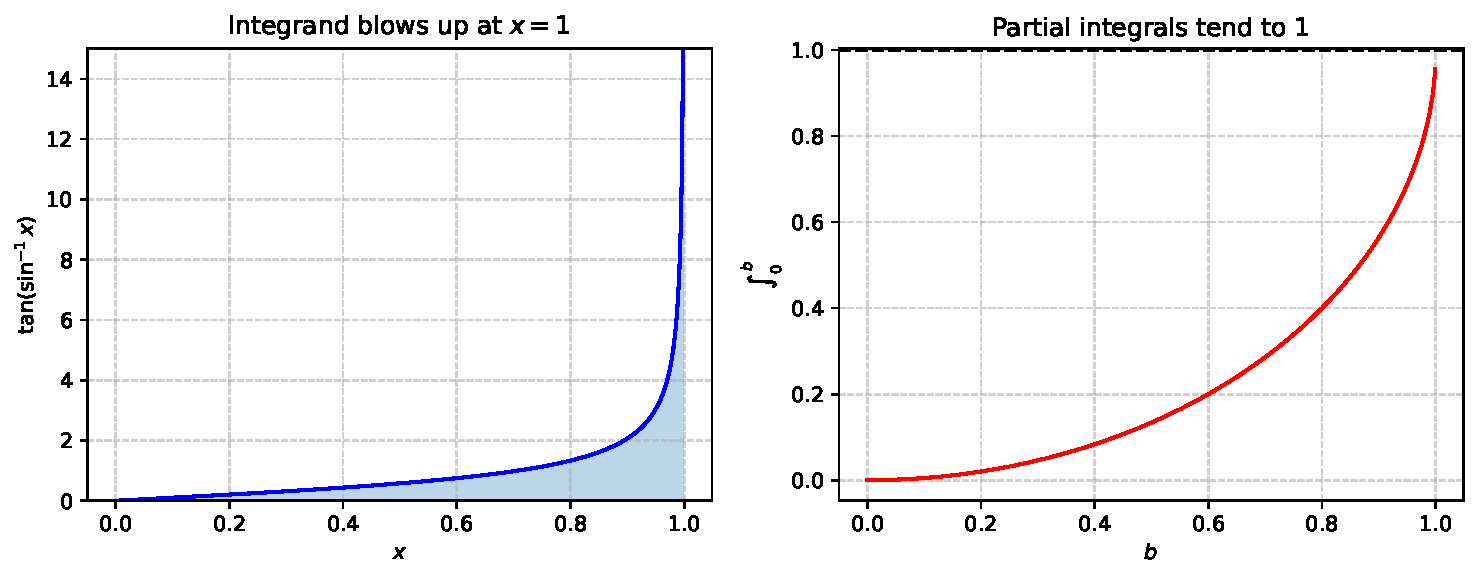
\includegraphics[width=0.95\linewidth]{figs/cbXIIq6.pdf}
    \caption{The integrand and the partial integrals $\int_0^b$ tending to $1$}
    \label{fig:EE26BTECH11218-cb12_q6}
\end{figure}
\item $\displaystyle\int\frac{e^x}{x+1}\sbrak{1+\brak{x+1}\log\brak{x+1}}dx$ equals
\begin{enumerate}[label=\alph*), itemsep=0pt]
    \begin{multicols}{4}
        \item $\frac{e^x}{x+1}+c$
        \item $e^x\frac{x}{x+1}+c$
        \item $e^x\log\brak{x+1}+e^x+c$
        \item $e^x\log\brak{x+1}+c$
    \end{multicols}
\end{enumerate}
\hfill (CBSE~XII~\cbxiiyear)
\\
\solution
The integrand is
\begin{align}
\frac{e^x}{x+1}\sbrak{1+\brak{x+1}\log\brak{x+1}} &= e^x\sbrak{\log\brak{x+1}+\frac{1}{x+1}} \\
&= e^x\brak{f+f'}, \quad f\brak{x}=\log\brak{x+1}
\end{align}
From \eqref{eq:EE26BTECH11218-cb12-expf},
\begin{align}
\int e^x\brak{f+f'}dx = e^xf+c = e^x\log\brak{x+1}+c
\end{align}
Hence the answer is option (d). Numerically, only option (d) has $F\brak{b}-F\brak{0}$ equal to $\int_0^b$ of the integrand (for $b=1$ both are $1.8842$). The following code verifies this in \figref{fig:EE26BTECH11218-cb12_q7}.
\begin{lstlisting}[frame=single, basicstyle=\rmfamily, escapeinside={(*@}{@*)}]
(*@\makebox[\dimexpr\linewidth-2\fboxsep-2\fboxrule\relax][c]{codes/cbXIIq7.py}@*)
\end{lstlisting}
\begin{figure}[H]
    \centering
    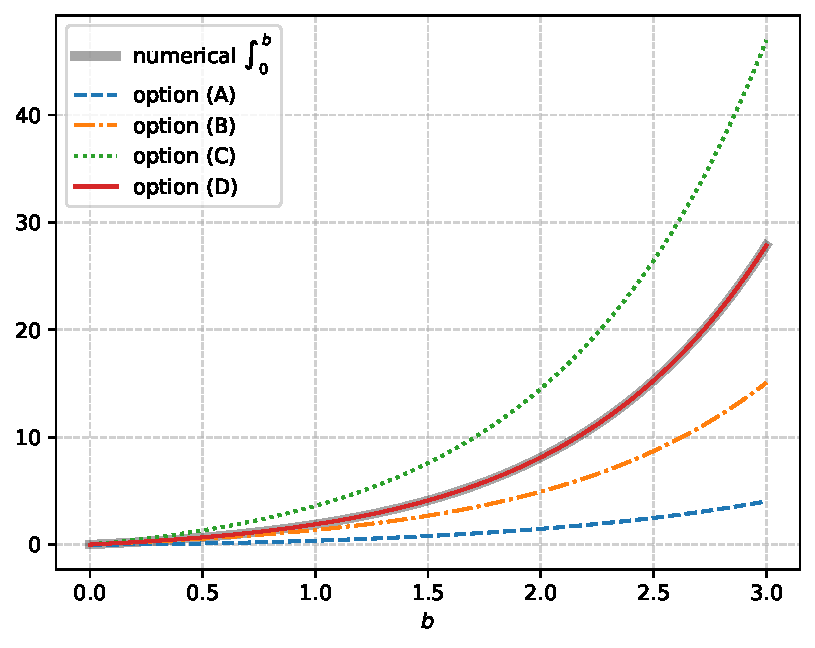
\includegraphics[width=0.70\linewidth]{figs/cbXIIq7.pdf}
    \caption{Numerical $\int_0^b$ compared with the increments of the four options}
    \label{fig:EE26BTECH11218-cb12_q7}
\end{figure}
\item The integrating factor of the differential equation $x\diff{y}{x}-y=\log x$ is \underline{\hspace{2cm}}.
\hfill (CBSE~XII~\cbxiiyear)
\\
\solution
In the form $\diff{y}{x}+Py=Q$ we have $P=-\frac{1}{x}$ and $Q=\frac{\log x}{x}$. From \eqref{eq:EE26BTECH11218-cb12-linode},
\begin{align}
\mu\brak{x} = e^{\int P\,dx} = e^{-\log x} = \frac{1}{x}
\end{align}
Then $\diff{}{x}\brak{\frac{y}{x}}=\frac{\log x}{x^2}$, and integrating by parts,
\begin{align}
\frac{y}{x} = -\frac{\log x+1}{x}+C \implies y = -\log x-1+Cx
\end{align}
The integrating factor is $\frac{1}{x}$. The following code verifies this with a numerical solution of the ODE in \figref{fig:EE26BTECH11218-cb12_q14}.
\begin{lstlisting}[frame=single, basicstyle=\rmfamily, escapeinside={(*@}{@*)}]
(*@\makebox[\dimexpr\linewidth-2\fboxsep-2\fboxrule\relax][c]{codes/cbXIIq14.py}@*)
\end{lstlisting}
\begin{figure}[H]
    \centering
    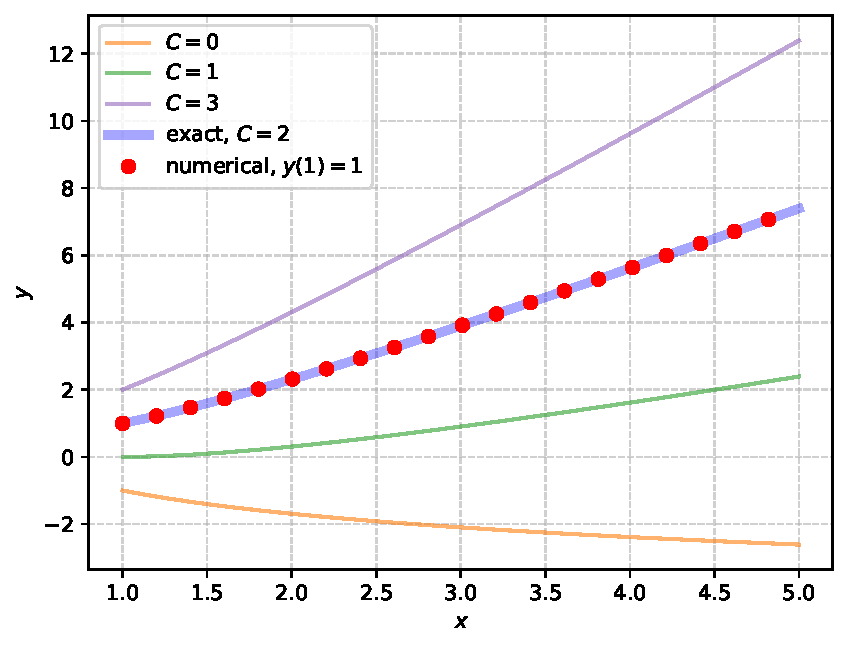
\includegraphics[width=0.70\linewidth]{figs/cbXIIq14.pdf}
    \caption{Numerical solution with $y\brak{1}=1$ (so $C=2$) against the closed form}
    \label{fig:EE26BTECH11218-cb12_q14}
\end{figure}
\item From a pack of $52$ cards, $3$ cards are drawn at random (without replacement). The probability that they are two red cards and one black card is \underline{\hspace{2cm}}.
\hfill (CBSE~XII~\cbxiiyear)
\\
\solution
Let $X$ be the number of red cards among the three drawn. From \eqref{eq:EE26BTECH11218-cb12-hyper} with $M=52$, $K=26$, $n=3$,
\begin{align}
\pr{X=2} = \frac{\binom{26}{2}\binom{26}{1}}{\binom{52}{3}} = \frac{325\times26}{22100} = \frac{13}{34}
\end{align}
The complete PMF is
\begin{align}
\brak{p_X\brak{0},\ p_X\brak{1},\ p_X\brak{2},\ p_X\brak{3}} = \brak{\frac{2}{17},\ \frac{13}{34},\ \frac{13}{34},\ \frac{2}{17}}
\end{align}
which sums to $1$. The following code verifies this in \figref{fig:EE26BTECH11218-cb12_q15}.
\begin{lstlisting}[frame=single, basicstyle=\rmfamily, escapeinside={(*@}{@*)}]
(*@\makebox[\dimexpr\linewidth-2\fboxsep-2\fboxrule\relax][c]{codes/cbXIIq15.py}@*)
\end{lstlisting}
\begin{figure}[H]
    \centering
    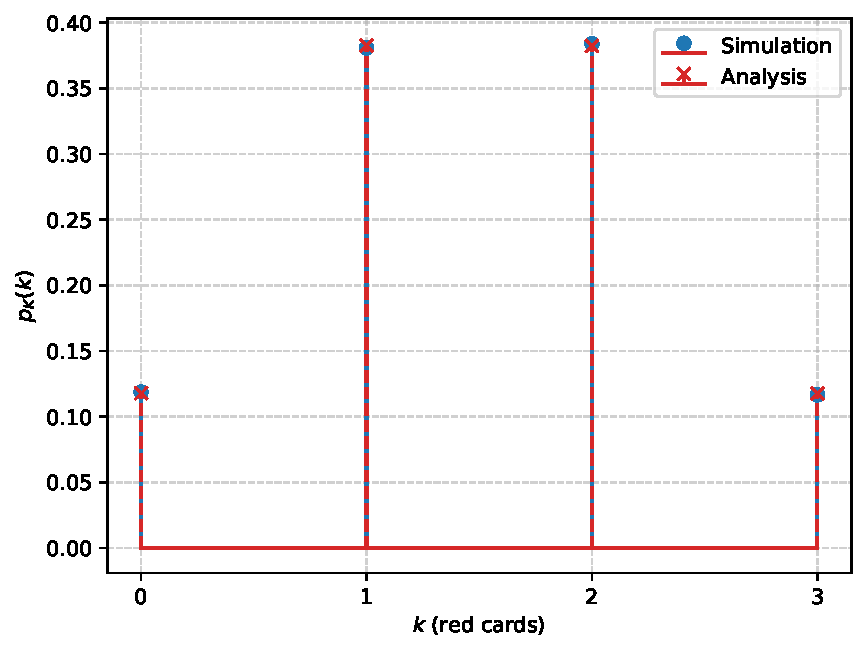
\includegraphics[width=0.70\linewidth]{figs/cbXIIq15.pdf}
    \caption{PMF of the number of red cards in three draws: Simulation vs Analysis}
    \label{fig:EE26BTECH11218-cb12_q15}
\end{figure}
\item If $\myvec{4 & x+2 \\ 2x-3 & x+1}$ is a symmetric matrix, then find the value of $x$.
\hfill (CBSE~XII~\cbxiiyear)
\\
\solution
Let the matrix be $\vec{A}$. From \eqref{eq:EE26BTECH11218-cb12-symskew}, the skew-symmetric part is
\begin{align}
\vec{K} = \frac{\vec{A}-\vec{A}^{\top}}{2} = \frac{5-x}{2}\myvec{0 & 1 \\ -1 & 0}
\end{align}
since $\brak{x+2}-\brak{2x-3}=5-x$. The matrix is symmetric iff $\vec{K}=\vec{0}$,
\begin{align}
5-x=0 \implies x=5, \qquad \vec{A} = \myvec{4 & 7 \\ 7 & 6}
\end{align}
The following code verifies this in \figref{fig:EE26BTECH11218-cb12_q19a}.
\begin{lstlisting}[frame=single, basicstyle=\rmfamily, escapeinside={(*@}{@*)}]
(*@\makebox[\dimexpr\linewidth-2\fboxsep-2\fboxrule\relax][c]{codes/cbXIIq19a.py}@*)
\end{lstlisting}
\begin{figure}[H]
    \centering
    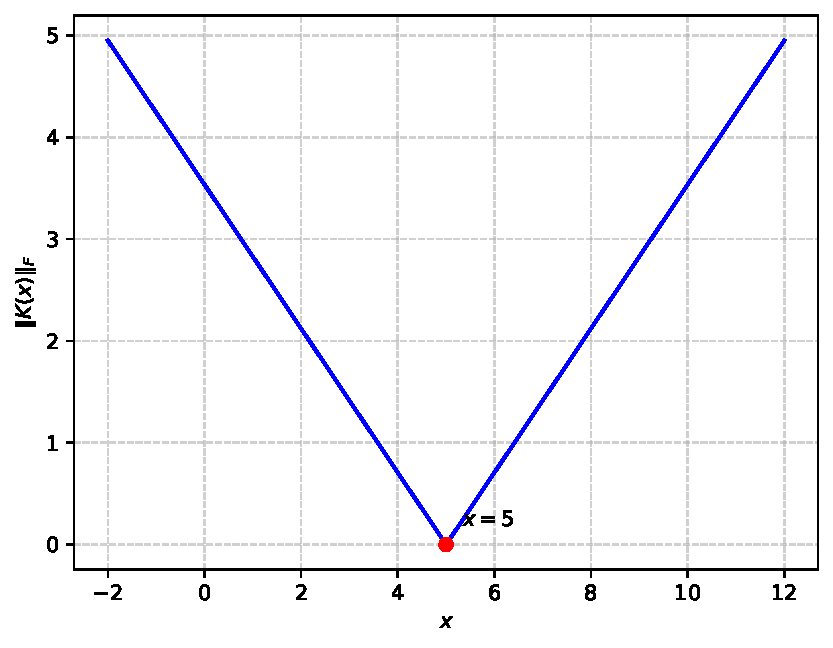
\includegraphics[width=0.70\linewidth]{figs/cbXIIq19a.pdf}
    \caption{Norm of the skew-symmetric part $\vec{K}\brak{x}$, zero at $x=5$}
    \label{fig:EE26BTECH11218-cb12_q19a}
\end{figure}
\item If $\vec{A}$ is a square matrix such that $\vec{A}^2=\vec{A}$, then find $\brak{2\vec{I}+\vec{A}}^3-19\vec{A}$.
\hfill (CBSE~XII~\cbxiiyear)
\\
\solution
Let $p\brak{\lambda}=\brak{2+\lambda}^3-19\lambda=\lambda^3+6\lambda^2-7\lambda+8$. Dividing by $\lambda^2-\lambda$,
\begin{align}
p\brak{\lambda} = \brak{\lambda^2-\lambda}\brak{\lambda+7}+8
\end{align}
so $r_1=0$ and $r_0=8$. Since $\vec{A}^2-\vec{A}=\vec{0}$, from \eqref{eq:EE26BTECH11218-cb12-idem},
\begin{align}
\brak{2\vec{I}+\vec{A}}^3-19\vec{A} = \brak{\vec{A}^2-\vec{A}}\brak{\vec{A}+7\vec{I}}+8\vec{I} = 8\vec{I}
\end{align}
This agrees with the eigenvalues of $\vec{A}$ being $0$ or $1$, where $p\brak{0}=p\brak{1}=8$. The following code verifies this for an orthogonal and an oblique projection matrix in \figref{fig:EE26BTECH11218-cb12_q19b}.
\begin{lstlisting}[frame=single, basicstyle=\rmfamily, escapeinside={(*@}{@*)}]
(*@\makebox[\dimexpr\linewidth-2\fboxsep-2\fboxrule\relax][c]{codes/cbXIIq19b.py}@*)
\end{lstlisting}
\begin{figure}[H]
    \centering
    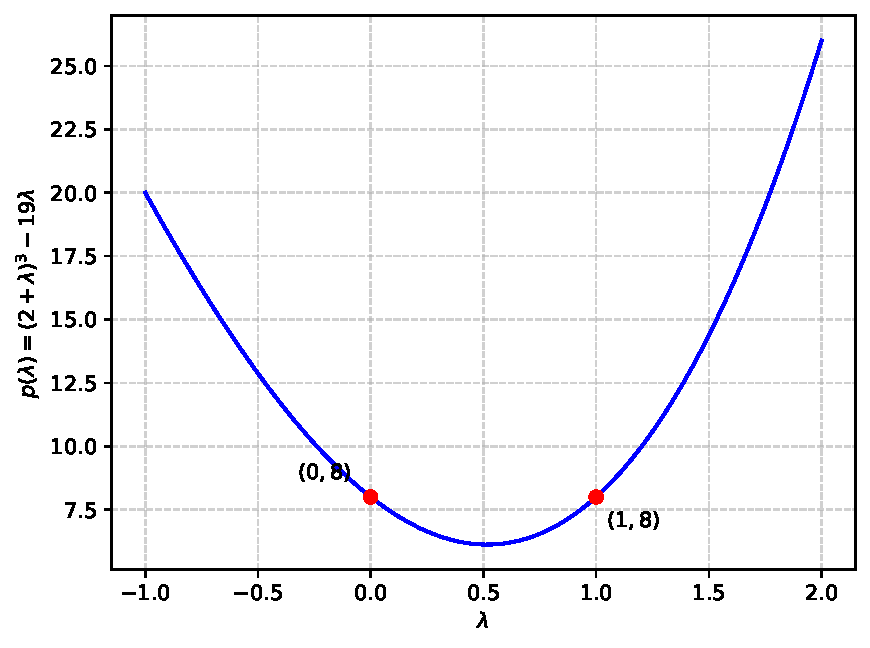
\includegraphics[width=0.70\linewidth]{figs/cbXIIq19b.pdf}
    \caption{$p\brak{\lambda}=\brak{2+\lambda}^3-19\lambda$ takes the value $8$ at $\lambda=0$ and $\lambda=1$}
    \label{fig:EE26BTECH11218-cb12_q19b}
\end{figure}
\item Let $W$ denote the set of words in the English dictionary. Define the relation $R$ by $R=\cbrak{\brak{x,y}\in W\times W : x \text{ and } y \text{ have at least one letter in common}}$. Show that $R$ is reflexive and symmetric, but not transitive.
\hfill (CBSE~XII~\cbxiiyear)
\\
\solution
From \eqref{eq:EE26BTECH11218-cb12-relation}, take $\vec{M}=\brak{\vec{L}\vec{L}^{\top}>0}$, where $L_{ik}=1$ iff word $i$ contains letter $k$.
\begin{enumerate}
\item \textbf{Reflexive:} $\brak{\vec{L}\vec{L}^{\top}}_{ii}=\sum_kL_{ik}^2$ is the number of distinct letters of word $i$, which is at least $1$ for every word, so $M_{ii}=1$.
\item \textbf{Symmetric:} $\vec{L}\vec{L}^{\top}$ is symmetric, so $\vec{M}=\vec{M}^{\top}$.
\item \textbf{Not transitive:} take $x=$ ``at'', $y=$ ``tip'', $z=$ ``pin''. The words ``at'' and ``tip'' share $t$, and ``tip'' and ``pin'' share $i,p$, so $\brak{\vec{M}^2}_{xz}>0$. But ``at'' and ``pin'' have no common letter, so $M_{xz}=0$ and $\brak{\vec{M}^2>0}\not\subseteq\brak{\vec{M}>0}$.
\end{enumerate}
The following code verifies this on a small set of words in \figref{fig:EE26BTECH11218-cb12_q21a}.
\begin{lstlisting}[frame=single, basicstyle=\rmfamily, escapeinside={(*@}{@*)}]
(*@\makebox[\dimexpr\linewidth-2\fboxsep-2\fboxrule\relax][c]{codes/cbXIIq21a.py}@*)
\end{lstlisting}
\begin{figure}[H]
    \centering
    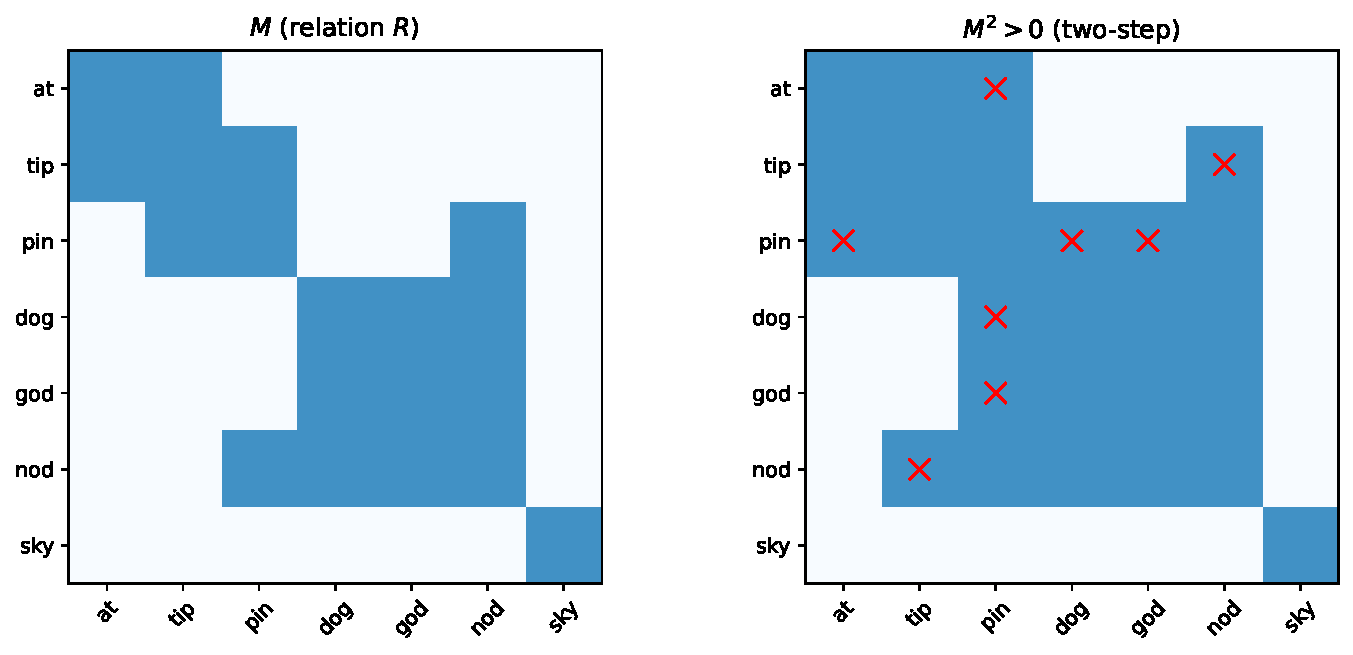
\includegraphics[width=0.85\linewidth]{figs/cbXIIq21a.pdf}
    \caption{$\vec{M}$ and $\brak{\vec{M}^2>0}$ for a few words; crosses mark violations of transitivity}
    \label{fig:EE26BTECH11218-cb12_q21a}
\end{figure}
\item For the matrix $\vec{A}=\myvec{2 & 3 \\ -4 & -6}$, verify $\vec{A}\brak{\mathrm{adj}\,\vec{A}} = \brak{\mathrm{adj}\,\vec{A}}\vec{A} = \abs{\vec{A}}\vec{I}$.
\hfill (CBSE~XII~\cbxiiyear)
\\
\solution
Here $\mathrm{tr}\brak{\vec{A}} = 2-6 = -4$ and $\abs{\vec{A}} = -12+12 = 0$, so $\vec{A}$ is singular and the inverse formula cannot be used. From \eqref{eq:EE26BTECH11218-cb12-ch}, Cayley-Hamilton gives
\begin{align}
\vec{A}^2+4\vec{A} = \vec{0}
\end{align}
(which can be checked directly: $\vec{A}^2=\myvec{-8 & -12 \\ 16 & 24}=-4\vec{A}$). From \eqref{eq:EE26BTECH11218-cb12-adj},
\begin{align}
\mathrm{adj}\,\vec{A} = -4\vec{I}-\vec{A} = \myvec{-6 & -3 \\ 4 & 2}
\end{align}
which is the transposed cofactor matrix. Then
\begin{align}
\vec{A}\brak{\mathrm{adj}\,\vec{A}} &= -4\vec{A}-\vec{A}^2 = -\brak{\vec{A}^2+4\vec{A}} = \vec{0} = \abs{\vec{A}}\vec{I} \\
\brak{\mathrm{adj}\,\vec{A}}\vec{A} &= -4\vec{A}-\vec{A}^2 = \vec{0} = \abs{\vec{A}}\vec{I}
\end{align}
Geometrically, the columns of $\mathrm{adj}\,\vec{A}$ are multiples of $\brak{3,\ -2}^{\top}$, which spans the null space of $\vec{A}$, so $\vec{A}$ maps them to $\vec{0}$. The following code verifies this in \figref{fig:EE26BTECH11218-cb12_q22}.
\begin{lstlisting}[frame=single, basicstyle=\rmfamily, escapeinside={(*@}{@*)}]
(*@\makebox[\dimexpr\linewidth-2\fboxsep-2\fboxrule\relax][c]{codes/cbXIIq22.py}@*)
\end{lstlisting}
\begin{figure}[H]
    \centering
    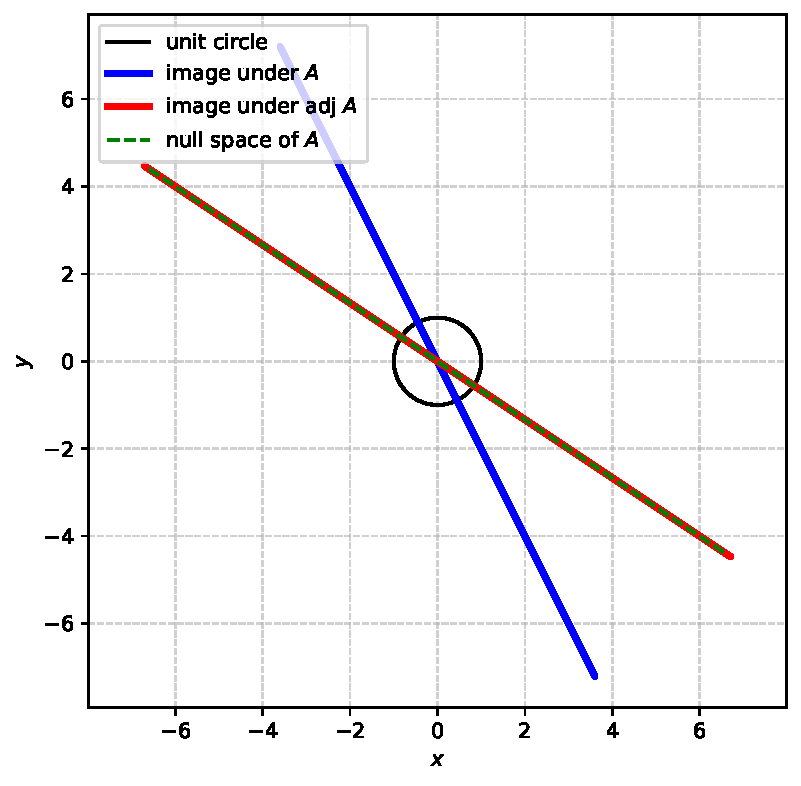
\includegraphics[width=0.70\linewidth]{figs/cbXIIq22.pdf}
    \caption{Images of the unit circle under $\vec{A}$ and $\mathrm{adj}\,\vec{A}$; the latter lies in the null space of $\vec{A}$}
    \label{fig:EE26BTECH11218-cb12_q22}
\end{figure}
\item A bag contains $19$ tickets numbered $1$ to $19$. A ticket is drawn at random and then another ticket is drawn without replacing the first one. Find the probability distribution of the number of even numbers on the tickets.
\hfill (CBSE~XII~\cbxiiyear)
\\
\solution
Let $X$ be the number of even tickets. Among $1,\dots,19$ there are $9$ even and $10$ odd tickets, so from \eqref{eq:EE26BTECH11218-cb12-hyper} with $M=19$, $K=9$, $n=2$,
\begin{align}
p_X\brak{k} = \frac{\binom{9}{k}\binom{10}{2-k}}{\binom{19}{2}}, \quad \binom{19}{2}=171
\end{align}
\begin{center}
\begin{tabular}{|c|c|c|c|}
\hline
$k$ & $0$ & $1$ & $2$ \\ \hline
$p_X\brak{k}$ & $\frac{45}{171}=\frac{5}{19}$ & $\frac{90}{171}=\frac{10}{19}$ & $\frac{36}{171}=\frac{4}{19}$ \\ \hline
\end{tabular}
\end{center}
The probabilities sum to $1$, and the mean is $E\sbrak{X}=\frac{2\cdot9}{19}=\frac{18}{19}$. The following code verifies this in \figref{fig:EE26BTECH11218-cb12_q26a}.
\begin{lstlisting}[frame=single, basicstyle=\rmfamily, escapeinside={(*@}{@*)}]
(*@\makebox[\dimexpr\linewidth-2\fboxsep-2\fboxrule\relax][c]{codes/cbXIIq26a.py}@*)
\end{lstlisting}
\begin{figure}[H]
    \centering
    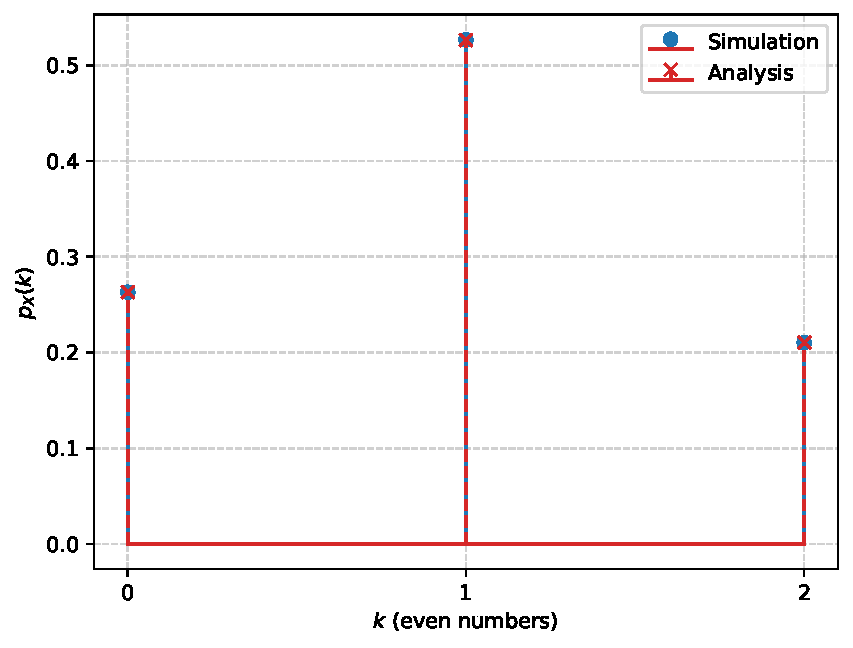
\includegraphics[width=0.70\linewidth]{figs/cbXIIq26a.pdf}
    \caption{PMF of the number of even tickets: Simulation vs Analysis}
    \label{fig:EE26BTECH11218-cb12_q26a}
\end{figure}
\item Find the probability distribution of the number of successes in two tosses of a die, where a success is defined as ``number greater than $5$''.
\hfill (CBSE~XII~\cbxiiyear)
\\
\solution
A success is the face $6$, so $p=\frac{1}{6}$. Let $X$ be the number of successes in $n=2$ independent tosses. From \eqref{eq:EE26BTECH11218-cb12-binom},
\begin{align}
p_X\brak{k} = \binom{2}{k}\brak{\frac{1}{6}}^k\brak{\frac{5}{6}}^{2-k}
\end{align}
\begin{center}
\begin{tabular}{|c|c|c|c|}
\hline
$k$ & $0$ & $1$ & $2$ \\ \hline
$p_X\brak{k}$ & $\frac{25}{36}$ & $\frac{10}{36}=\frac{5}{18}$ & $\frac{1}{36}$ \\ \hline
\end{tabular}
\end{center}
This is also the convolution $\brak{\frac{5}{6},\ \frac{1}{6}}*\brak{\frac{5}{6},\ \frac{1}{6}}$, with mean $np=\frac{1}{3}$ and variance $np\brak{1-p}=\frac{5}{18}$. The following code verifies this in \figref{fig:EE26BTECH11218-cb12_q26b}.
\begin{lstlisting}[frame=single, basicstyle=\rmfamily, escapeinside={(*@}{@*)}]
(*@\makebox[\dimexpr\linewidth-2\fboxsep-2\fboxrule\relax][c]{codes/cbXIIq26b.py}@*)
\end{lstlisting}
\begin{figure}[H]
    \centering
    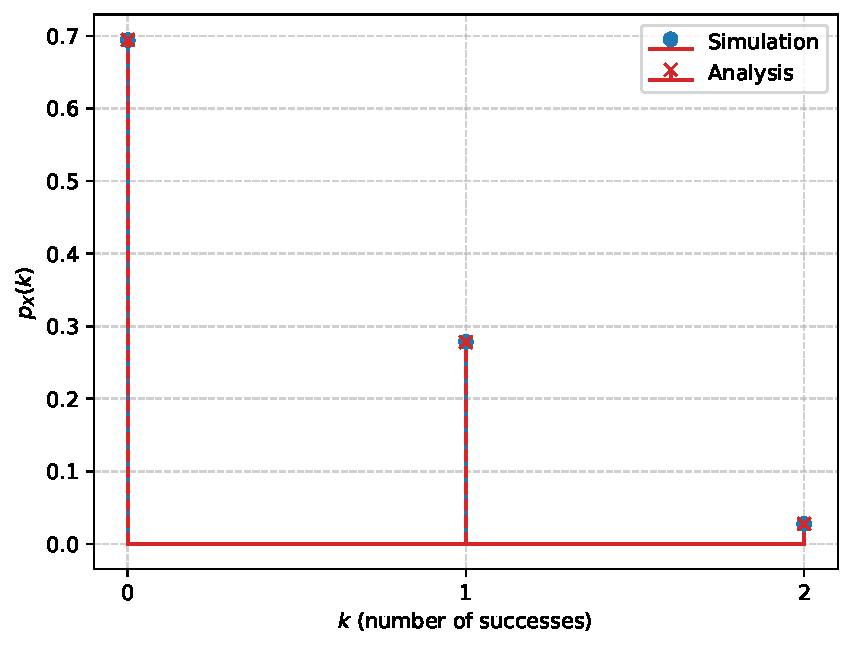
\includegraphics[width=0.70\linewidth]{figs/cbXIIq26b.pdf}
    \caption{PMF of the number of sixes in two tosses: Simulation vs Analysis}
    \label{fig:EE26BTECH11218-cb12_q26b}
\end{figure}
\item Find the equation of the line joining $A\brak{1,3}$ and $B\brak{0,0}$ using determinants. Also find $k$ if $D\brak{k,0}$ is a point such that the area of $\triangle ABD$ is $3$ square units.
\hfill (CBSE~XII~\cbxiiyear)
\\
\solution
From \eqref{eq:EE26BTECH11218-cb12-det}, the line $AB$ is
\begin{align}
\mydet{x & y & 1 \\ 1 & 3 & 1 \\ 0 & 0 & 1} = x\brak{3-0}-y\brak{1-0}+1\brak{0-0} = 3x-y = 0
\end{align}
The area of $\triangle ABD$ is
\begin{align}
\Delta = \frac{1}{2}\abs{\mydet{1 & 3 & 1 \\ 0 & 0 & 1 \\ k & 0 & 1}} = \frac{1}{2}\abs{3k} = 3 \implies \abs{k}=2
\end{align}
\begin{align}
\therefore k = \pm2
\end{align}
The following code verifies this in \figref{fig:EE26BTECH11218-cb12_q28b}.
\begin{lstlisting}[frame=single, basicstyle=\rmfamily, escapeinside={(*@}{@*)}]
(*@\makebox[\dimexpr\linewidth-2\fboxsep-2\fboxrule\relax][c]{codes/cbXIIq28b.py}@*)
\end{lstlisting}
\begin{figure}[H]
    \centering
    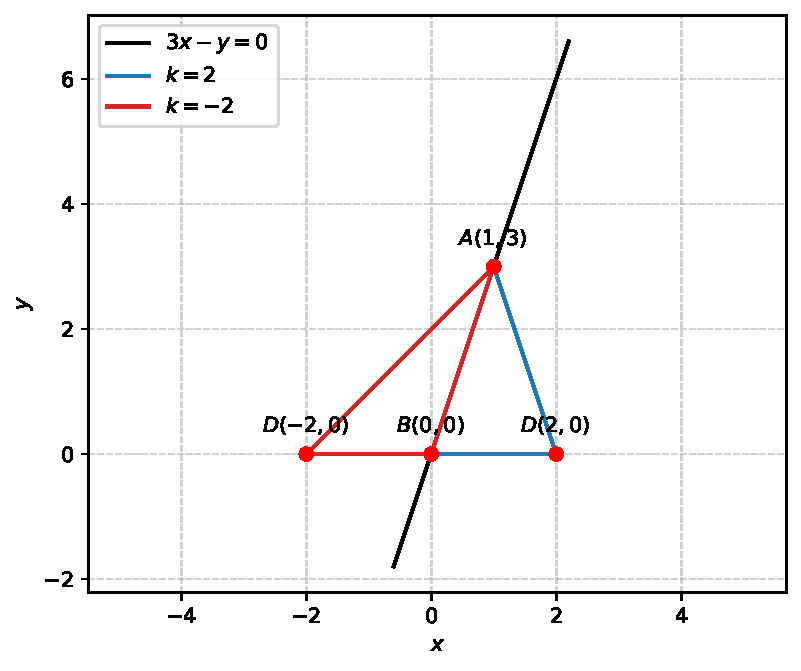
\includegraphics[width=0.70\linewidth]{figs/cbXIIq28b.pdf}
    \caption{The line $3x-y=0$ and the triangles $ABD$ for $k=\pm2$}
    \label{fig:EE26BTECH11218-cb12_q28b}
\end{figure}
\item Prove that three points $A$, $B$ and $C$ with position vectors $\vec{a}$, $\vec{b}$ and $\vec{c}$ respectively are collinear if and only if $\brak{\vec{b}\times\vec{c}}+\brak{\vec{c}\times\vec{a}}+\brak{\vec{a}\times\vec{b}}=\vec{0}$.
\hfill (CBSE~XII~\cbxiiyear)
\\
\solution
Let $\vec{S}=\vec{b}\times\vec{c}+\vec{c}\times\vec{a}+\vec{a}\times\vec{b}$. From \eqref{eq:EE26BTECH11218-cb12-cross},
\begin{align}
\vec{S} = \brak{\vec{b}-\vec{a}}\times\brak{\vec{c}-\vec{a}}
\end{align}
This vanishes iff $\vec{b}-\vec{a}$ and $\vec{c}-\vec{a}$ are parallel, that is (for $A\ne B$) iff $\vec{c}-\vec{a}=\kappa\brak{\vec{b}-\vec{a}}$ for some $\kappa$, which says that $C$ lies on the line $AB$. If $A=B$ both statements hold trivially. Hence $A,B,C$ are collinear iff $\vec{S}=\vec{0}$. Moreover $\norm{\vec{S}}=2\,\mathrm{area}\brak{\triangle ABC}$.

For $\vec{a}=\brak{1,\ 0,\ 2}^{\top}$ and $\vec{b}=\brak{3,\ 1,\ 1}^{\top}$, the point $\vec{c}=\vec{a}+2.5\brak{\vec{b}-\vec{a}}$ gives $\vec{S}=\vec{0}$, while $\vec{c}=\brak{2,\ 3,\ 4}^{\top}$ gives $\vec{S}=\brak{5,\ -5,\ 5}^{\top}$ and $\frac{1}{2}\norm{\vec{S}}=4.33$, which equals the area from Heron's formula. The following code verifies this in \figref{fig:EE26BTECH11218-cb12_q29}.
\begin{lstlisting}[frame=single, basicstyle=\rmfamily, escapeinside={(*@}{@*)}]
(*@\makebox[\dimexpr\linewidth-2\fboxsep-2\fboxrule\relax][c]{codes/cbXIIq29.py}@*)
\end{lstlisting}
\begin{figure}[H]
    \centering
    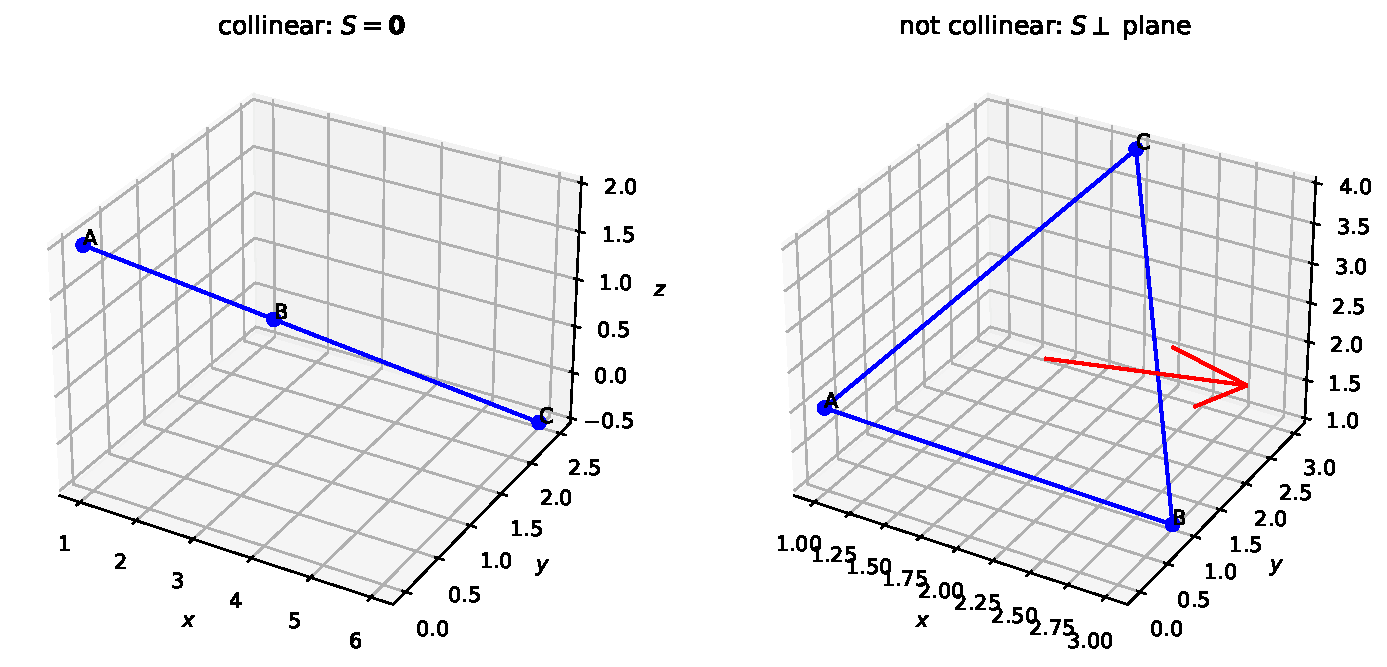
\includegraphics[width=0.95\linewidth]{figs/cbXIIq29.pdf}
    \caption{Collinear points ($\vec{S}=\vec{0}$) and a triangle with $\vec{S}$ normal to its plane}
    \label{fig:EE26BTECH11218-cb12_q29}
\end{figure}
\item Find the shortest distance between the lines $\frac{x-1}{2}=\frac{y+1}{3}=z$ and $\frac{x+1}{5}=\frac{y-2}{1},\ z=2$, and hence write whether the lines are intersecting or not.
\hfill (CBSE~XII~\cbxiiyear)
\\
\solution
From \eqref{eq:EE26BTECH11218-cb12-symm}, the lines are $\vec{x}=\vec{a}_1+s\vec{m}_1$ and $\vec{x}=\vec{a}_2+t\vec{m}_2$ with
\begin{align}
\vec{a}_1 = \myvec{1 \\ -1 \\ 0}, \ \vec{m}_1 = \myvec{2 \\ 3 \\ 1}, \qquad &\vec{a}_2 = \myvec{-1 \\ 2 \\ 2}, \ \vec{m}_2 = \myvec{5 \\ 1 \\ 0} \\
\vec{b} = \vec{a}_2-\vec{a}_1 &= \myvec{-2 \\ 3 \\ 2}
\end{align}
The normal equations in \eqref{eq:EE26BTECH11218-cb12-skew} are
\begin{align}
\myvec{14 & 13 \\ 13 & 26}\myvec{s \\ -t} = \myvec{7 \\ -7} \implies s=\frac{7}{5}, \quad t=\frac{63}{65}
\end{align}
The closest points are $\brak{3.8,\ 3.2,\ 1.4}^{\top}$ on the first line and $\brak{3.846,\ 2.969,\ 2}^{\top}$ on the second. The distance is $\norm{\vec{M}\vec{z}-\vec{b}}$, and from \eqref{eq:EE26BTECH11218-cb12-skew-cross}, with $\vec{m}_1\times\vec{m}_2=\brak{-1,\ 5,\ -13}^{\top}$ and $\vec{b}^{\top}\brak{\vec{m}_1\times\vec{m}_2}=-9$,
\begin{align}
d = \frac{\abs{-9}}{\sqrt{195}} = \frac{9}{\sqrt{195}} \approx 0.645
\end{align}
Since $d\ne0$, the lines do \textbf{not} intersect (they are skew). The following code verifies this in \figref{fig:EE26BTECH11218-cb12_q30a}.
\begin{lstlisting}[frame=single, basicstyle=\rmfamily, escapeinside={(*@}{@*)}]
(*@\makebox[\dimexpr\linewidth-2\fboxsep-2\fboxrule\relax][c]{codes/cbXIIq30a.py}@*)
\end{lstlisting}
\begin{figure}[H]
    \centering
    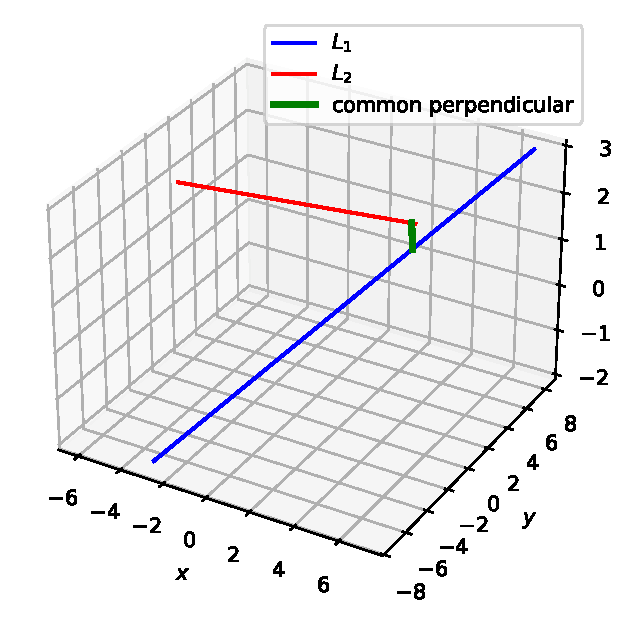
\includegraphics[width=0.80\linewidth]{figs/cbXIIq30a.pdf}
    \caption{Skew lines and their common perpendicular}
    \label{fig:EE26BTECH11218-cb12_q30a}
\end{figure}
\item Find the equation of the plane through the line of intersection of the planes $\vec{r}\cdot\brak{\hat{i}+3\hat{j}}+6=0$ and $\vec{r}\cdot\brak{3\hat{i}-\hat{j}-4\hat{k}}=0$, which is at a unit distance from the origin.
\hfill (CBSE~XII~\cbxiiyear)
\\
\solution
The planes are $\vec{n}_1^{\top}\vec{x}+e_1=0$ and $\vec{n}_2^{\top}\vec{x}+e_2=0$ with
\begin{align}
\vec{n}_1 = \myvec{1 \\ 3 \\ 0}, \ e_1=6, \qquad \vec{n}_2 = \myvec{3 \\ -1 \\ -4}, \ e_2=0
\end{align}
From \eqref{eq:EE26BTECH11218-cb12-pencil}, the planes through the line of intersection have $\vec{n}=\vec{n}_1+\lambda\vec{n}_2$ and $e=6$. From \eqref{eq:EE26BTECH11218-cb12-plane-dist}, the distance from the origin is $1$ iff $\norm{\vec{n}}^2=e^2$,
\begin{align}
\norm{\vec{n}_1+\lambda\vec{n}_2}^2 = \vec{n}_1^{\top}\vec{n}_1+2\lambda\vec{n}_1^{\top}\vec{n}_2+\lambda^2\vec{n}_2^{\top}\vec{n}_2 = 10+0+26\lambda^2 = 36 \implies \lambda=\pm1
\end{align}
\begin{align}
\lambda=1: \ 4x+2y-4z+6=0 \implies 2x+y-2z+3=0 \\
\lambda=-1: \ -2x+4y+4z+6=0 \implies x-2y-2z-3=0
\end{align}
Both are at distance $\frac{3}{3}=1$ from the origin. The following code verifies this in \figref{fig:EE26BTECH11218-cb12_q30b}.
\begin{lstlisting}[frame=single, basicstyle=\rmfamily, escapeinside={(*@}{@*)}]
(*@\makebox[\dimexpr\linewidth-2\fboxsep-2\fboxrule\relax][c]{codes/cbXIIq30b.py}@*)
\end{lstlisting}
\begin{figure}[H]
    \centering
    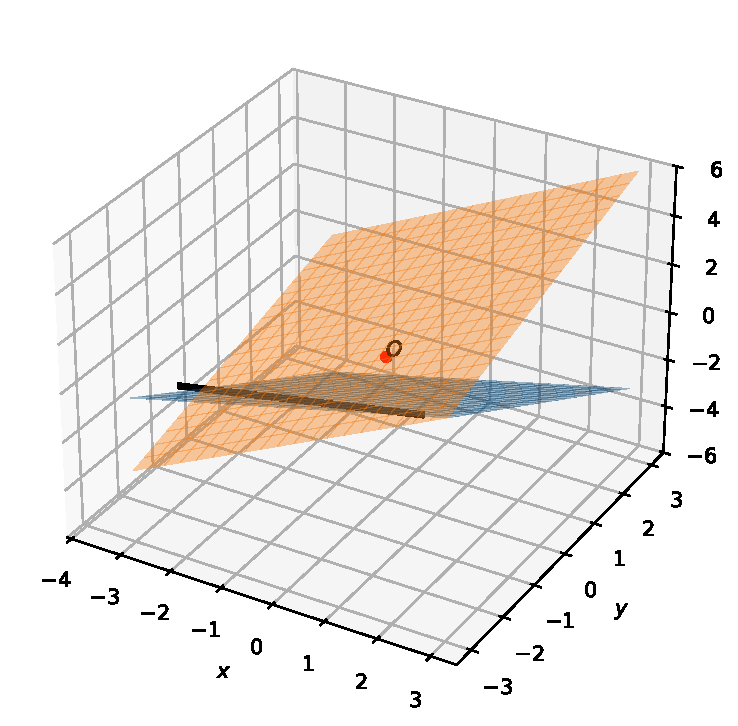
\includegraphics[width=0.80\linewidth]{figs/cbXIIq30b.pdf}
    \caption{The two required planes and the line of intersection of the given planes}
    \label{fig:EE26BTECH11218-cb12_q30b}
\end{figure}
\item A bag contains $5$ red and $4$ black balls, and a second bag contains $3$ red and $6$ black balls. One of the two bags is selected at random and two balls are drawn at random (without replacement), both of which are found to be red. Find the probability that these two balls are drawn from the second bag.
\hfill (CBSE~XII~\cbxiiyear)
\\
\solution
Let $B_i$ be the event that bag $i$ is chosen, with $\pr{B_i}=\frac{1}{2}$, and let $E$ be the event that both balls are red. From \eqref{eq:EE26BTECH11218-cb12-hyper},
\begin{align}
\pr{E\mid B_1} = \frac{\binom{5}{2}}{\binom{9}{2}} = \frac{10}{36}, \qquad \pr{E\mid B_2} = \frac{\binom{3}{2}}{\binom{9}{2}} = \frac{3}{36}
\end{align}
From \eqref{eq:EE26BTECH11218-cb12-bayes},
\begin{align}
\pr{B_2\mid E} = \frac{\frac{1}{2}\cdot\frac{3}{36}}{\frac{1}{2}\cdot\frac{10}{36}+\frac{1}{2}\cdot\frac{3}{36}} = \frac{3}{13}
\end{align}
The following code verifies this in \figref{fig:EE26BTECH11218-cb12_q32}.
\begin{lstlisting}[frame=single, basicstyle=\rmfamily, escapeinside={(*@}{@*)}]
(*@\makebox[\dimexpr\linewidth-2\fboxsep-2\fboxrule\relax][c]{codes/cbXIIq32.py}@*)
\end{lstlisting}
\begin{figure}[H]
    \centering
    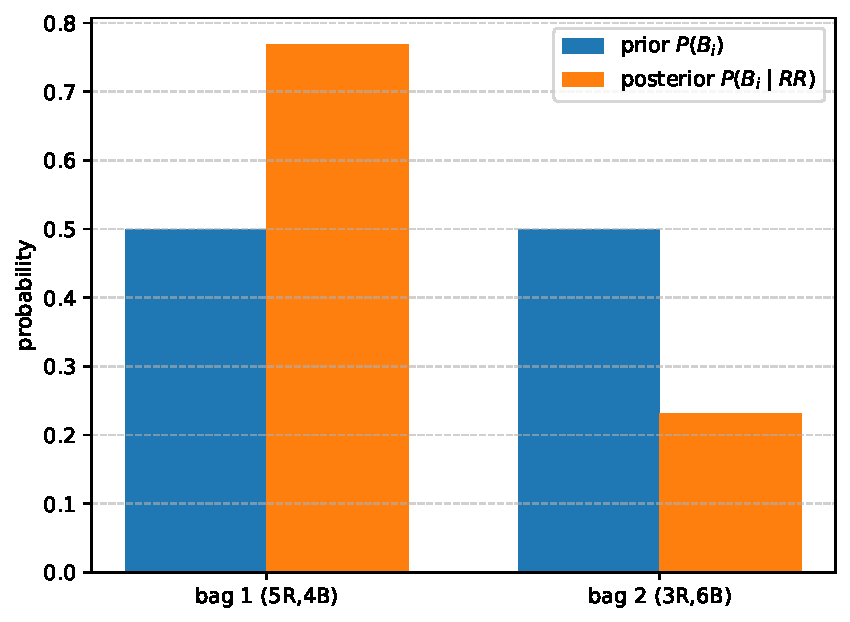
\includegraphics[width=0.70\linewidth]{figs/cbXIIq32.pdf}
    \caption{Prior and posterior probabilities of the two bags}
    \label{fig:EE26BTECH11218-cb12_q32}
\end{figure}
\item If the area between the curves $x=y^2$ and $x=4$ is divided into two equal parts by the line $x=a$, then find the value of $a$ using integration.
\hfill (CBSE~XII~\cbxiiyear)
\\
\solution
From \eqref{eq:EE26BTECH11218-cb12-area}, the total area is $A\brak{4}=\frac{4}{3}\cdot4^{3/2}=\frac{32}{3}$. The line $x=a$ halves it iff
\begin{align}
A\brak{a} = \frac{4}{3}a^{3/2} = \frac{1}{2}\cdot\frac{32}{3} \implies a^{3/2} = 4
\end{align}
\begin{align}
\therefore a = 4^{2/3} = 2^{4/3} \approx 2.52
\end{align}
The following code solves $A\brak{a}=\frac{1}{2}A\brak{4}$ numerically and verifies this in \figref{fig:EE26BTECH11218-cb12_q35a}.
\begin{lstlisting}[frame=single, basicstyle=\rmfamily, escapeinside={(*@}{@*)}]
(*@\makebox[\dimexpr\linewidth-2\fboxsep-2\fboxrule\relax][c]{codes/cbXIIq35a.py}@*)
\end{lstlisting}
\begin{figure}[H]
    \centering
    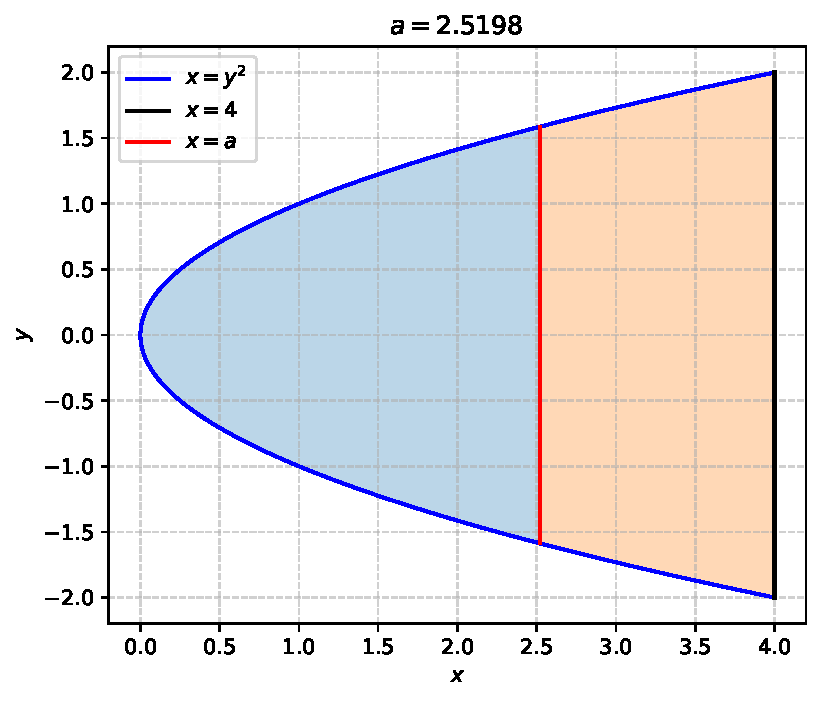
\includegraphics[width=0.70\linewidth]{figs/cbXIIq35a.pdf}
    \caption{Region between $x=y^2$ and $x=4$ divided equally by $x=a$}
    \label{fig:EE26BTECH11218-cb12_q35a}
\end{figure}
\item Find $\displaystyle\int\frac{x}{\brak{x-1}^2\brak{x+2}}dx$.
\hfill (CBSE~XII~\cbxiiyear)
\\
\solution
From \eqref{eq:EE26BTECH11218-cb12-partial}, $x = A\brak{x-1}\brak{x+2}+B\brak{x+2}+C\brak{x-1}^2$. Matching the coefficients of $x^2$, $x$ and $1$,
\begin{align}
\myvec{1 & 0 & 1 \\ 1 & 1 & -2 \\ -2 & 2 & 1}\myvec{A \\ B \\ C} = \myvec{0 \\ 1 \\ 0} \implies \myvec{A \\ B \\ C} = \myvec{\frac{2}{9} \\ \frac{1}{3} \\ -\frac{2}{9}}
\end{align}
Hence
\begin{align}
\int\frac{x\,dx}{\brak{x-1}^2\brak{x+2}} = \frac{2}{9}\ln\abs{x-1}-\frac{1}{3\brak{x-1}}-\frac{2}{9}\ln\abs{x+2}+c
\end{align}
The following code verifies this, including $\int_2^5=0.4337$ against the antiderivative, in \figref{fig:EE26BTECH11218-cb12_q35b}.
\begin{lstlisting}[frame=single, basicstyle=\rmfamily, escapeinside={(*@}{@*)}]
(*@\makebox[\dimexpr\linewidth-2\fboxsep-2\fboxrule\relax][c]{codes/cbXIIq35b.py}@*)
\end{lstlisting}
\begin{figure}[H]
    \centering
    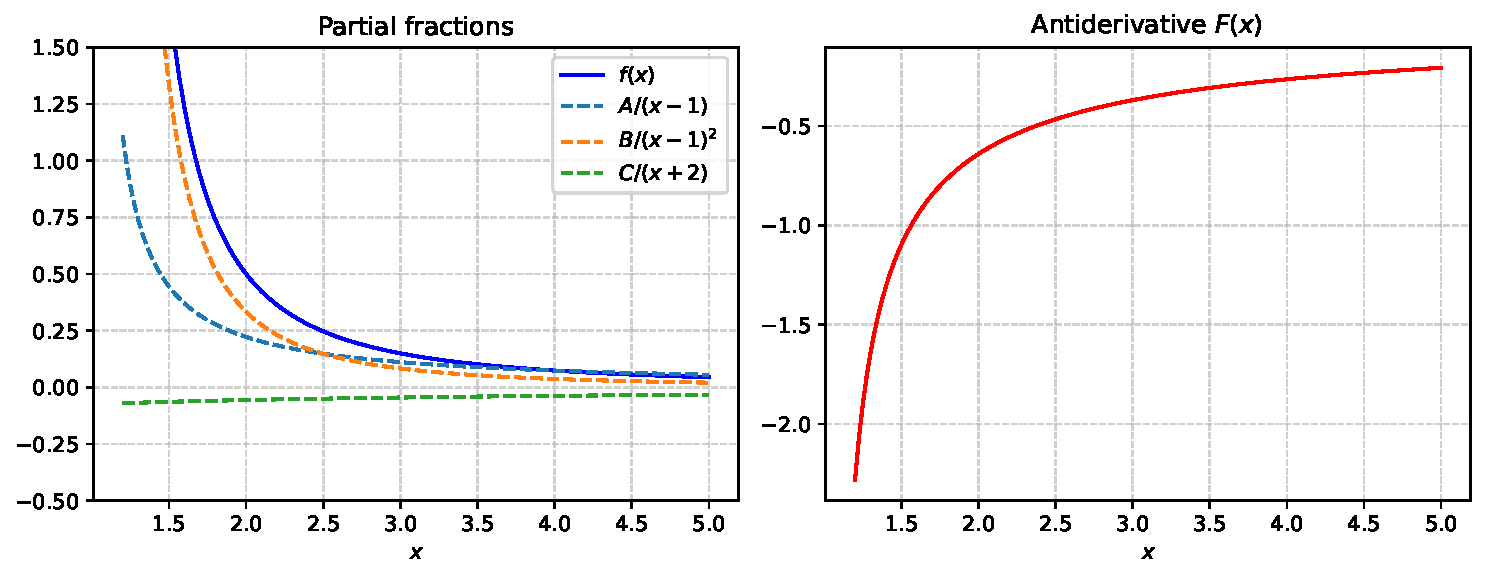
\includegraphics[width=0.95\linewidth]{figs/cbXIIq35b.pdf}
    \caption{Partial fractions of the integrand and its antiderivative}
    \label{fig:EE26BTECH11218-cb12_q35b}
\end{figure}
\end{enumerate}

\end{document}
